---
id: two-points-to-the-goal
title: Two Points to the Goal: A Noise-Conditioned Mixture Density Network for Probabilistic Penalty Kick Prediction
date: 2026-11-09
authors: Jiahe Zhu、Zixuan Chen、Jiachen Xiao（上海交通大学）
venue: UPC 2026 · Problem B · 队号 155
summary: 只给两次早期坐标，预测足球在门线上的落点并给出不确定度：122.5 万条物理仿真轨迹 + 条件于测量噪声的 Wiener 残差混合密度网络，5 mm 噪声下众数 (2.67, 1.79) m，浏览器里可实时重现。
abstract: 从罚球点到球门的两次早期观测，估计足球穿过门面时的位置并量化不确定度。我们在重力、二次阻力与马格努斯升力下积分弹道，用 122.5 万条仿真轨迹（含 Asai 弧线球等实测锚点）训练条件于测量噪声的残差混合密度网络：5 mm 坐标噪声下众数为 (Y, Z) = (2.67, 1.79) m，50% 与 95% 区域面积 0.106 与 0.619 m²，门框内概率 97.7%。在 109,108 条留出弹道上中位误差 0.266 m，名义 50% 与 95% 区间的实测覆盖为 50.1% 与 95.1%。
tags: [点球, 足球空气动力学, 马格努斯力, 混合密度网络, 不确定性量化, 概率预测, UPC]
---
% 站点副本：逐字取自 UPC 2026 B 题队伍 155 的作者版 TeX（paper/main_authors.tex），
% 仅做网页排版适配：文档头与摘要移入元信息、公式改为 KaTeX 的 $$ 形式（故去编号，
% 两处 \eqref 改为文字指代）、图/表编号与 \ref \cite 显式化、图径改为站内资源、
% 去掉印刷分页与浮动体命令。原始 PDF 保存在 assets/papers/two-points-to-the-goal/。
\href{assets/papers/two-points-to-the-goal/two-points-to-the-goal.pdf}{下载论文全文（PDF）}

\section*{Abstract}

From two early positions of a penalty kick, we estimate where the ball crosses the goal plane and quantify uncertainty. We integrate gravity, quadratic drag and Magnus lift, then train a noise-conditioned residual mixture density network on airborne trajectories drawn from a mixture of uniform launches and priors informed by tracked flights, including Asai's curve kicks.

For the stated kick at an assumed $5\,\mathrm{mm}$ coordinate noise, the model gives a mode of $(Y,Z)=(2.67,1.79)\,\mathrm{m}$ and joint $50\%$ and $95\%$ region areas of $0.106$ and $0.619\,\mathrm{m^2}$. Conditional on airborne crossing, the estimated probability of crossing within a goal rectangle inset by one ball radius is $97.7\%$. In a Bayesian sensitivity check at the same noise level, changing the launch prior from uniform to the v3 mixture raised the conditional in-frame probability from $91.5\%$ to $96.6\%$.

Of $1{,}225{,}000$ simulated launches, $1{,}091{,}052$ cross in flight. On $109{,}108$ held-out airborne crossings simulated under the same launch mixture and flight model, the median error is $0.266\,\mathrm{m}$ at $5\,\mathrm{mm}$, and the nominal $50\%$ and $95\%$ regions cover $50.1\%$ and $95.1\%$. In a separate paired experiment with one training seed and a specified simulated surface, including rebound and rolling crossings in training reduces median error on post-contact crossings from $0.242$ to $0.163\,\mathrm{m}$ at $5\,\mathrm{mm}$.

\noindent\textbf{Keywords:} penalty kick; football aerodynamics; Magnus lift;
mixture density network; uncertainty quantification; probabilistic trajectory forecasting

\section{1 Introduction}
\subsection{1.1 Problem Restatement}

Take the penalty spot as the origin and the goal as the rectangle $|Y|<3.66\,\mathrm{m}$, $0<Z<2.44\,\mathrm{m}$ in the plane $x=11\,\mathrm{m}$ [1]. From $\mathbf r(0)=(0,0,0.11)\,\mathrm{m}$ and two later observations, the problem asks for the most likely crossing point and its uncertainty. The stated case gives [2]

$$
\mathbf r(0.05)=(1.50,0.45,0.44)\,\mathrm{m},\qquad
  \mathbf r(0.10)=(2.96,0.86,0.74)\,\mathrm{m}.
$$

Unknown spin and aerodynamic forces make extrapolation from two points ambiguous. With a fixed start, $5\,\mathrm{mm}$ independent coordinate errors give a second-difference acceleration uncertainty of $4.47\,\mathrm{m\,s^{-2}}$. For the stated kick, the same noise gives a median radial deviation of about $0.34\,\mathrm{m}$ under quadratic extrapolation (Appendix~A).

\subsection{1.2 Background and Approach}

Wind-tunnel tests of non-spinning balls found drag coefficients near $0.43$ and $0.15$ on either side of the drag crisis, at Reynolds numbers around $2.2$--$3.0\times10^5$ [3]. A later ball comparison reached $3.3\times10^5$ [4]. Free-kick fits give $C_D=0.25$--$0.30$. In the same study ten free kicks had speeds of $23.0$--$28.3\,\mathrm{m\,s^{-1}}$ at $0.1\,\mathrm{s}$ [8]. Trajectory studies find lift coefficients of order $0.2$--$0.3$ under some conditions and estimate aerodynamic curves from tracked flights [6, 7]. These results inform our choices of prior bounds and lift law.

We compare a quadratic extrapolation, a Bayesian reference and an MDN [19] under shared flight dynamics. We fit simulation priors using tracked Asai, ISSIA-3D and DFL trajectories and digitised Barber--Carr\'e data [5, 15, 16, 17, 18]. Held-out simulations assess coverage. We assess transfer to the three Asai kicks using reduced-mixture models trained without their anchors.

\section{2 Materials and Methods}
\subsection{2.1 Assumptions and Approximations}

Forecasts use the known start, fixed observation times and specified coordinate noise $\sigma$. The main endpoint distribution conditions on reaching the goal plane before ground contact, denoted by $\mathcal E$. Section~3.7 also considers crossings after ground contact. We report the density mode for the stated case and use the mean for point-error scoring. We score geometric in-frame arrival when the ball centre crosses within $|Y|\le 3.55\,\mathrm{m}$ and $0.11\le Z\le 2.33\,\mathrm{m}$, allowing one ball radius at each boundary.

\begin{itemize}
  \item \textbf{A1.} \textbf{Ball.} A rigid sphere has mass $0.430\,\mathrm{kg}$, radius $0.110\,\mathrm{m}$ and cross-section $A_{\mathrm{ball}}=\pi R^2$ [1]. Buoyancy is omitted (Section~2.2).
  \item \textbf{A2.} \textbf{Air.} The main model uses still air at $\rho_{\mathrm{air}}=1.20\,\mathrm{kg\,m^{-3}}$.
  \item \textbf{A3.} \textbf{Drag.} Each flight has a constant $C_D$ in $[0.15,0.30]$, a range that includes reported free-kick and supercritical wind-tunnel estimates [3, 8].
  \item \textbf{A4.} \textbf{Lift.} Transverse spin determines lift. The slope and cap in the lift law below are chosen to match the measured order of magnitude [3, 6].
  \item \textbf{A5.} \textbf{Spin.} We hold spin fixed, following the short-flight approximation discussed by Team~358 [9]. Section~3.6 tests a $0.5\,\mathrm{s}$ decay time.
  \item \textbf{A6.} \textbf{Measurement.} The start is exact. The two observations have independent Gaussian coordinate errors with common standard deviation $\sigma\in\{2,5,10,15\}\,\mathrm{mm}$ in evaluation. The supplied coordinates are reported to the nearest centimetre, but their measurement accuracy is unspecified. We use $5\,\mathrm{mm}$, half the reporting increment, as a reference value for the assumed coordinate standard deviation and examine values from $2$ to $15\,\mathrm{mm}$. If rounding alone gives a uniform error, its maximum magnitude is $5\,\mathrm{mm}$ and its standard deviation is about $2.9\,\mathrm{mm}$. We choose $5\,\mathrm{mm}$ as a conservative reference to allow for possible tracking and digitisation errors; it is not a measured standard deviation.
  \item \textbf{A7.} \textbf{Prior.} Table~1 gives the common simulation bounds. The Bayesian reference uses independent uniforms and the main training set uses the mixture in Section~2.5.
\end{itemize}

\begin{table}[htbp]
  
  \caption{Table 1. Launch-parameter bounds for the simulation. Uniform reference draws are independent within these bounds.}
  \begin{tabular}{lcc}
    \toprule
    Parameter & Lower & Upper \\
    \midrule
    $v_x$ ($\mathrm{m\,s^{-1}}$) & 18 & 35 \\
    $v_y$ ($\mathrm{m\,s^{-1}}$) & $-12$ & 12 \\
    $v_z$ ($\mathrm{m\,s^{-1}}$) & 0.5 & 12 \\
    $\omega_x,\omega_y,\omega_z$ ($\mathrm{rad\,s^{-1}}$) & $-60$ & 60 \\
    $C_D$ & 0.15 & 0.30 \\
    \bottomrule
  \end{tabular}
\end{table}

\subsection{2.2 Physical Model}

Let $\mathbf u=\mathbf v-\mathbf w$ be the velocity relative to air, $\mathbf g=-g\hat{\mathbf z}$ with $g=9.81\,\mathrm{m\,s^{-2}}$, and $V=4\pi R^3/3$. The force balance combines weight, quadratic drag, transverse lift and Archimedean buoyancy [10, 11, 12, 13].

$$
m\dot{\mathbf v}=m\mathbf g-\tfrac12\rho_{\mathrm{air}} A_{\mathrm{ball}} C_D|\mathbf u|\mathbf u
  +\tfrac12\rho_{\mathrm{air}} A_{\mathrm{ball}} C_L|\mathbf u|^2\hat{\mathbf n}-\rho_{\mathrm{air}} V\mathbf g.
$$

Buoyancy is $0.066\,\mathrm{N}$ upward, or $1.6\%$ of the ball's weight. Omitting it gives

$$
\begin{aligned}
\dot{\mathbf r}&=\mathbf v,\\
  \dot{\mathbf v}&=\mathbf g-\frac{\rho_{\mathrm{air}} A_{\mathrm{ball}} C_D}{2m}|\mathbf u|\mathbf u
    +\frac{\rho_{\mathrm{air}} A_{\mathrm{ball}} C_L}{2m}|\mathbf u|^2\hat{\mathbf n}.
\end{aligned}
$$

We use a three-dimensional spin vector $\boldsymbol\omega$ and define

$$
\hat{\mathbf{n}}=
  \begin{cases}
    \dfrac{\boldsymbol{\omega}\times\mathbf{u}}{|\boldsymbol{\omega}\times\mathbf{u}|}, & |\boldsymbol{\omega}\times\mathbf{u}|>0,\\[2mm]
    \mathbf{0}, & \text{otherwise},
  \end{cases}
  \qquad
  C_L=\min\!\left(1.4\,\frac{R\,|\boldsymbol{\omega}\times\mathbf{u}|}{|\mathbf{u}|^2},\,0.30\right).
$$

Spin about $+\hat{\mathbf z}$ gives the special case $\hat{\mathbf n}\propto\hat{\mathbf z}\times\mathbf u$. Lift vanishes when the cross product is zero. Bray and Kerwin give a related vector model for free kicks [8].

\subsection{2.3 Numerical Solution and Event Detection}

The synthetic flight simulator uses fourth-order Runge--Kutta (RK4), a $2\,\mathrm{ms}$ step and a $1.5\,\mathrm{s}$ horizon. Linear interpolation locates $x=11\,\mathrm{m}$ and $z=R$, retaining goal-plane crossings before contact. Reintegrating $1{,}024$ sampled launches per million-scale dataset at $1\,\mathrm{ms}$ leaves the crossing status unchanged and changes the recorded endpoints by at most about $0.012\,\mathrm{mm}$. The ISSIA model-form check uses \texttt{solve\_ivp}. Tracked-flight prefix forecasts use RK4 with a maximum $5\,\mathrm{ms}$ step.

\subsection{2.4 Bayesian Inference of Launch Conditions}

Let $\boldsymbol{\theta}=(\mathbf{v}_0,\boldsymbol{\omega},C_D)$ and let $\mathbf{y}_1,\mathbf{y}_2$ be the two observed positions. With the start fixed and independent Gaussian errors,

$$
p(\mathbf{y}_1,\mathbf{y}_2\mid\boldsymbol{\theta})
  =\prod_{i=1}^{2}\frac{1}{(2\pi\sigma^2)^{3/2}}
   \exp\!\left[-\frac{\|\mathbf{y}_i-\mathbf{r}(t_i;\boldsymbol{\theta})\|^2}{2\sigma^2}\right].
$$

Four-stage adaptive importance sampling combines a $20\%$ prior component with a Gaussian proposal. The first three stages use possibly widened likelihoods to adapt the proposal by weighted moments. The fourth stage alone supplies the posterior at the specified $\sigma$, with weights proportional to likelihood times $p(\boldsymbol\theta)/q(\boldsymbol\theta)$. We use $40{,}000$ draws per stage for the stated kick and report the conditional effective sample size (ESS). A weighted Gaussian kernel estimate on a $160\times160$ grid gives the mode and joint highest-density regions (HDRs) [24].

\subsection{2.5 Million-Scale Simulation Dataset}

We generate $1{,}225{,}000$ launches per sampling strategy. Before flight integration, the full mixture assigns $40\%$ to independent uniform draws, $24\%$ to two DFL penalty anchors, $12\%$ to three Asai curve-kick anchors and $24\%$ to aerodynamic anchors from eleven other DFL segments, three ISSIA arcs and one digitised Barber--Carr\'e trajectory. The frozen anchor records store the fitted seven-parameter vector, the number of frames used and the trajectory fit RMSE for each arc; the fitted vectors are listed in Table~16 (Appendix~C). The five penalty and curve-kick anchors supply both launch and aerodynamic parameters. Their perturbations are independent zero-mean Gaussians with standard deviations $(1.8,2.4,1.5,7.5,7.5,7.5,0.025)$ in the parameter order and units of Table~1. We use $(3.0,3.8,2.5,12,12,12,0.035)$ for $30\%$ of these draws. For the other fifteen anchors, half the forward speeds are uniform and half use a truncated normal with mean $28.5$ and standard deviation $3.2\,\mathrm{m\,s^{-1}}$. Lateral and vertical speeds use truncated normals with means $0$ and $5.5$ and standard deviations $6.5$ and $2.8\,\mathrm{m\,s^{-1}}$, respectively. We rotate fitted spin into the sampled horizontal heading, then add Gaussian noise with standard deviation $6\,\mathrm{rad\,s^{-1}}$ per spin component and $0.025$ in $C_D$. We clip to the bounds in Table~1. For a lateral reflection, we reverse the signs of $v_y$, $\omega_x$ and $\omega_z$.

We call the mixture sampling scheme without ballistic aiming v2; v3 adds ballistic aiming to the same base mixture. In v3, we select $65\%$ of the non-Asai anchor draws with $v_x\ge24\,\mathrm{m\,s^{-1}}$. For a nominal flight time $11/v_x$, we choose uniform ballistic targets in $Y\in[-3.85,3.85]\,\mathrm{m}$ and $Z\in[0.55,2.65]\,\mathrm{m}$ to set the transverse launch velocities. We rotate spin with the change in horizontal heading and integrate the full flight equations to obtain labels. The Asai holdout is a separate choice: in both \texttt{v2\_no\_asai} and \texttt{v3\_no\_asai}, we replace all Asai-derived draws with the same independent uniform draws, whereas \texttt{v3\_all} retains the Asai anchors. Below, a “v3 model” is a model trained on v3-generated data. The two given observations are used only for the final query and a descriptive count of nearby simulated prefixes.

\begin{table}[htbp]
  
  
  \caption{Table 2. Airborne crossings by split, from $1{,}225{,}000$ candidate launches per dataset. Splits are disjoint by trajectory and stratified by source anchor.}
  \begin{tabular}{lrrrrr}
    \toprule
    Dataset & Retained (\%) & Train & Selection & Calibration & Test \\
    \midrule
    \texttt{v3\_all} & 89.07 & 872,841 & 54,553 & 54,550 & 109,108 \\
    \texttt{v2\_no\_asai} & 83.52 & 818,534 & 51,161 & 51,157 & 102,314 \\
    \texttt{v3\_no\_asai} & 87.44 & 856,879 & 53,556 & 53,553 & 107,112 \\
    \bottomrule
  \end{tabular}
\end{table}

The calibration parameters for the full-mixture v3 model are listed in Table~17 (Appendix~C). The main v3 dataset retains $1{,}091{,}052$ airborne crossings. The splits are assigned before perturbing the observations, with approximate proportions of $80\%$, $5\%$, $5\%$ and $10\%$. At a six-coordinate Euclidean distance below $0.10\,\mathrm{m}$ from the given prefix, the full mixture has $1{,}761$ airborne neighbours. This count describes local sampling density. The unaimed source holdout falls below the design target of $85\%$ airborne retention and is kept as the exploratory sampling control.

Our first models used SiLU on smaller simulations [23]. We call the later frozen model developed on $50{,}000$ uniform-prior simulated trajectories v1: it uses 11 inputs, three 128-unit GELU layers and three Gaussian components to predict $(Y,Z)$ directly. We subsequently rebuilt the dataset and predictor using tracked-flight anchors, including Asai's measurements. The earlier datasets and model results are archived.

\subsection{2.6 Wiener Residual Mixture Density Network}

Let $\mathbf b_{\mathrm{lin}}$ be a gravity-only crossing estimate based on midpoint velocity and let $\mathbf b_{\mathrm{quad}}$ be a regularised quadratic estimate from the two observed positions and the known start. The feature extractor limits extrapolation times and uses the linear time estimate when the quadratic time is invalid. We blend the endpoints using a Wiener shrinkage weight,

$$
\mathbf b_\sigma=\mathbf b_{\mathrm{lin}}+w_\sigma
     (\mathbf b_{\mathrm{quad}}-\mathbf b_{\mathrm{lin}}),\qquad
  w_\sigma=\frac{s_*^2}{s_*^2+5\sigma^2/\Delta t^4},\qquad
  s_*=7.5\,\mathrm{m\,s^{-2}} .
$$

The denominator incorporates the second-difference acceleration variance (Appendix~A). The fixed scale $s_*$ sets the strength of shrinkage. The 22 features are the three midpoint velocity and three second-difference acceleration components, midpoint speed, the parallel component and three perpendicular components of gravity-corrected acceleration, its perpendicular magnitude, apparent drag and lift, two extrapolation times, four baseline endpoint coordinates, $w_\sigma$ and $\sigma$. Apparent drag and lift divide the negative parallel component and the perpendicular magnitude by $\rho_{\mathrm{air}} A_{\mathrm{ball}}|\mathbf v_{\rm mid}|^2/(2m)$, with clips of $[-2,3]$ and $[0,2]$, respectively. The extrapolators floor forward speed at $6\,\mathrm{m\,s^{-1}}$. The gravity-only time is clipped to $[0.20,1.20]\,\mathrm{s}$. The quadratic time must lie in $(0.18,1.15)\,\mathrm{s}$, with discriminant above $4\,\mathrm{m^2\,s^{-2}}$ and $|a_x|>10^{-4}\,\mathrm{m\,s^{-2}}$. Otherwise we evaluate the quadratic at the gravity-only time. Quadratic endpoints are clipped to $[-8,8]\,\mathrm{m}$ in $Y$ and $[-3,8]\,\mathrm{m}$ in $Z$. The features are standardised using training data.

A $192$-unit input projection and two $192$-unit residual blocks use LayerNorm and GELU [21, 22]. The head produces five correlated bivariate Gaussian components,

$$
p(\mathbf q\mid\mathbf y_1,\mathbf y_2,\sigma,\mathcal E)
    = \sum_{k=1}^{5} \pi_k
       \mathcal N\bigl(\mathbf q;\mathbf b_\sigma+\boldsymbol\delta_k,
                        \boldsymbol\Sigma_k\bigr),\qquad
       \mathbf q=(Y,Z).
$$

The six outputs per component give a softmax weight logit, a two-dimensional residual $\boldsymbol\delta_k$, two positive scales $s_{kj}=\operatorname{softplus}(r_{kj})+10^{-3}$ and correlation $\rho_k=0.98\tanh(r_{k\rho})$. The diagonal of $\boldsymbol\Sigma_k$ is $(s_{k1}^2,s_{k2}^2)$ and its off-diagonal entry is $\rho_k s_{k1}s_{k2}$.

Each dataset uses three runs (seeds 11, 42 and 155), AdamW with initial learning rate $0.002$ and cosine decay, batch size 512 and 100 epochs [14]. Each epoch draws a new $\sigma\sim U[1,18]\,\mathrm{mm}$ per trajectory and adds independent Gaussian noise to the six coordinates. We choose the checkpoint by selection-set negative log-likelihood (NLL). On the independent calibration fold, separately at each test noise level, we fit a common scale multiplier by NLL and adjust the nominal $50\%$ and $95\%$ highest-density region (HDR) thresholds using ranks from 256 predictive draws per flight [24, 26]. For each calibration example, the rank is the fraction of the 256 draws with density at or below the observed endpoint's density. For target coverage $c$, we use one minus the empirical $(1-c)$ quantile of these ranks as the adjusted mass, clipped to $[0.35,0.65]$ for $c=0.50$ and $[0.85,0.985]$ for $c=0.95$. The prediction region is the upper density level set enclosing the adjusted mass. We score physical-coordinate NLL, Euclidean errors of the predictive mean, and empirical coverage on the held-out test split. The data manifests record source and simulator hashes, split counts and dataset hashes. Computations use NumPy, SciPy, PyTorch and Matplotlib [27, 28, 29, 30].

\subsection{2.7 Comparison Protocol}

We repeat the model comparisons on fixed subsets of the v3 splits, drawing $65{,}536$ training, $4{,}096$ selection and $8{,}192$ test trajectories without replacement (seed 20261108). Each candidate uses the same 60-epoch budget, three training seeds and optimizer, with the specified interventions below. Checkpoint selection minimises mean selection NLL at 2, 5, 10 and $15\,\mathrm{mm}$. The full-mixture checkpoints supply the main forecast. They are scored on the same test subset as a reference trained with a larger budget.

Arms A and B use six coordinates plus $\sigma$. C and D use sixteen physical features, and E adds the quadratic endpoint to A's inputs. A and C predict absolute coordinates. B, D and E predict residuals about the quadratic endpoint, skip examples with no finite quadratic prediction during training, and use a zero endpoint in that case during evaluation. Arms A--E use the same three-layer, width-192 GELU body and five components. We also retrain the legacy coordinate MDN (two 64-unit SiLU layers, three components) and the Physics-Informed Residual Mixture Density Network (PI-ResMDN) on these v3 rows. PI-ResMDN uses three 128-unit SiLU layers, five components, and its original 16 features and quadratic fallback. Its physics-informed design combines velocity and acceleration features, including acceleration parallel and perpendicular to velocity, with learned output residuals added to a constant-acceleration crossing estimate.

For architecture screening, we compare 11 and 16 physical inputs for the direct target, and vary mixture size and depth using the 22-feature Wiener residual target. Depth is screened with SiLU. A shallower candidate is preferred when its NLL disadvantage is within one paired seed standard deviation and the mean absolute HDR coverage gap rises by at most 1.5 percentage points. We then compare activations at that depth. The intervention screen holds the three-layer v3 architecture fixed and changes only covariance correlation, the learning rate schedule, or the reuse of the initial noise draw for each trajectory.

\section{3 Results}

\subsection{3.1 Answer for the Stated Kick}

The quadratic baseline gives $T=0.405\,\mathrm{s}$ and $(Y,Z)=(2.495,1.920)\,\mathrm{m}$ (Appendix~A). At $\sigma=5\,\mathrm{mm}$, the calibrated full-mixture MDN (seed 11) gives a mode of $(2.67,1.79)\,\mathrm{m}$, versus $(2.65,2.05)\,\mathrm{m}$ for the uniform-prior Bayesian reference. Their mode heights differ by $0.26\,\mathrm{m}$, and their conditional in-frame probabilities under the same inset geometry are $97.7\%$ and $91.1\%$, respectively. The MDN mean is $(2.71,1.86)\,\mathrm{m}$. The mode heights for seeds 42 and 155 are approximately $1.83$ and $1.80\,\mathrm{m}$. The Bayesian joint region areas are $0.219$ and $0.809\,\mathrm{m^2}$ (ESS $2{,}893$). Both models use the same flight equations, and the comparison varies the launch distribution and density estimator jointly. The earlier v1 model gave a crossing-height mode of $2.15\,\mathrm{m}$ for this input at $5\,\mathrm{mm}$ noise.

In a separate control for this kick, we keep the simulator, likelihood and airborne-crossing condition fixed and compare independent uniforms with the v3 launch mixture. We bias the random inputs that generate launch velocities and correct for the proposal by importance weighting (four runs of $180{,}000$ draws per prior). Switching to v3 raises the conditional in-frame probability from $91.5\%$ to $96.6\%$ and moves the posterior mean height from $1.99$ to $1.86\,\mathrm{m}$. This accounts for most of the in-frame probability gap with the MDN in this case. The uniform-prior mode varies across runs and smoothing choices. The $91.1\%$ estimate from the earlier adaptive sampler and the pooled $91.5\%$ estimate agree within estimated Monte Carlo uncertainty.

\begin{figure}

\href{assets/papers/two-points-to-the-goal/case_regions_v3.png}{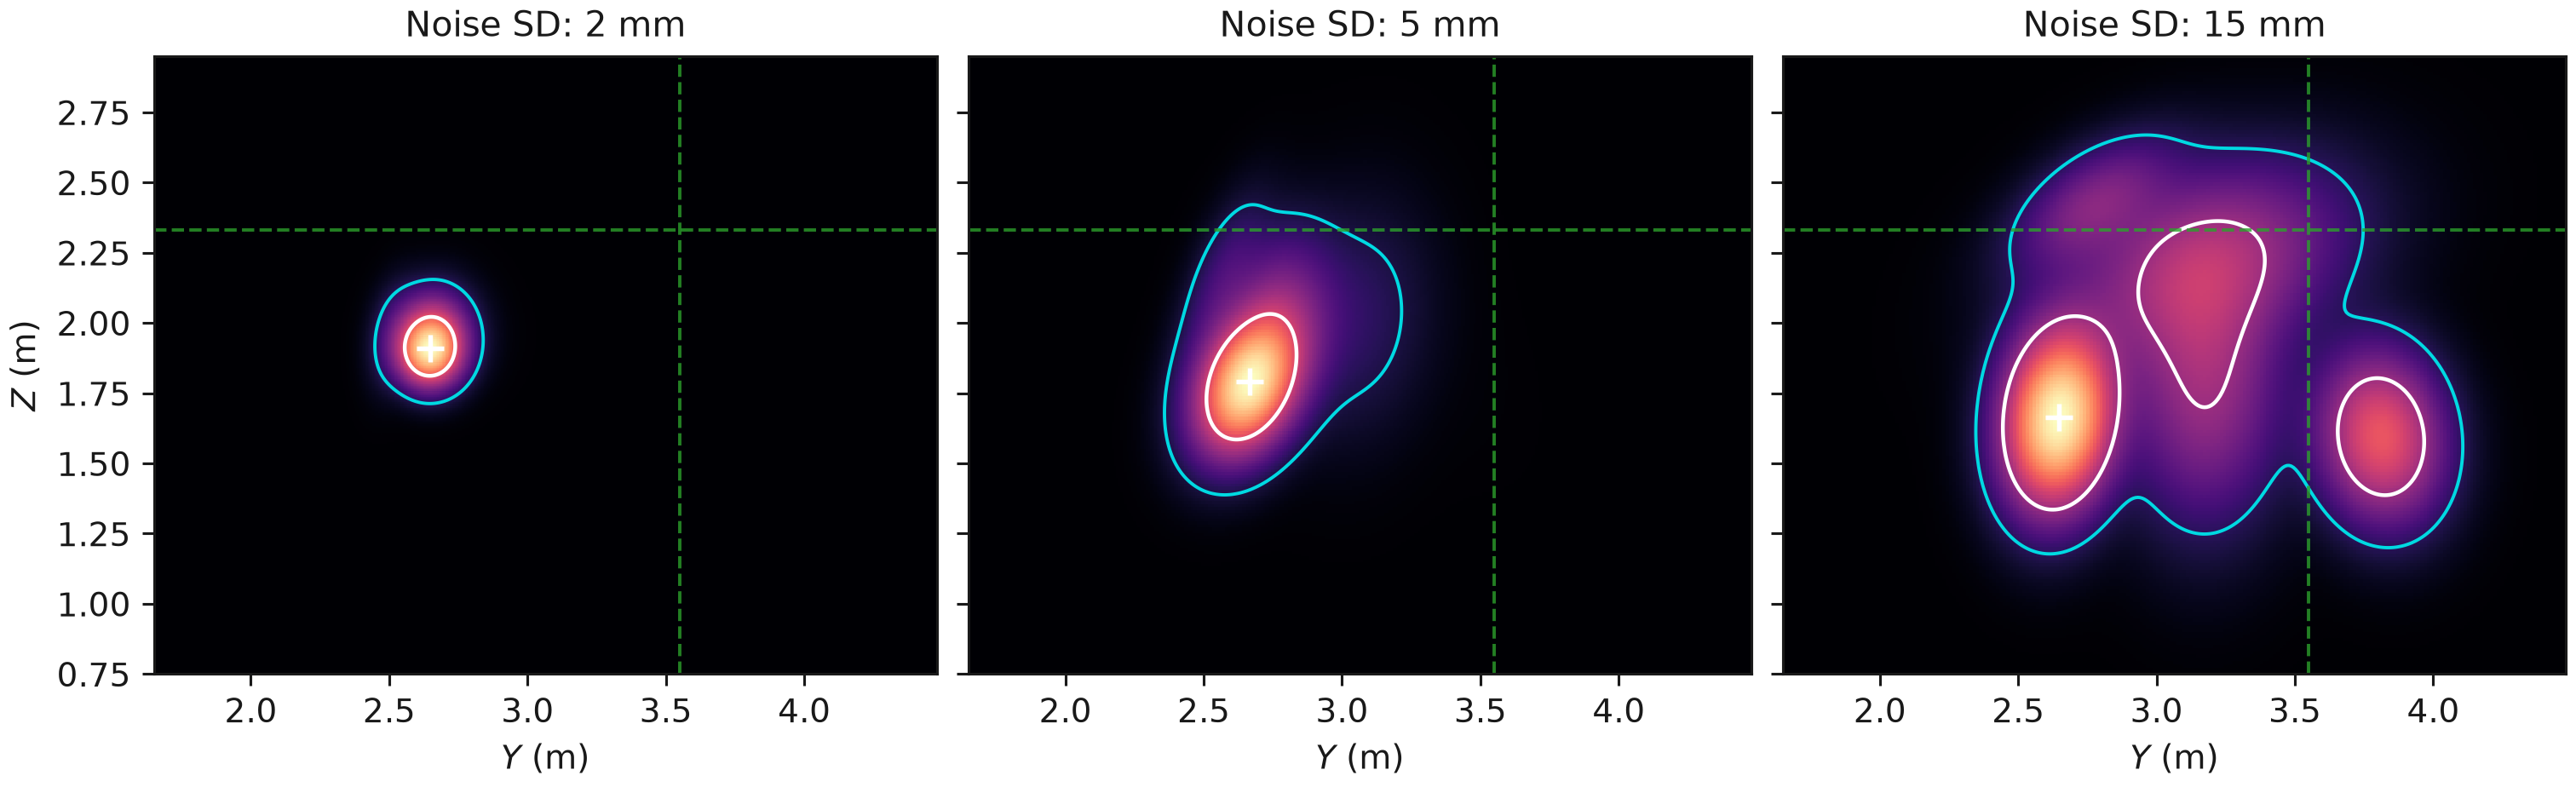
\includegraphics{assets/papers/two-points-to-the-goal/case_regions_v3.png}}
\caption{Fig. 1. Seed-11 density near the right side of the goal. White and cyan enclose the calibrated $50\%$ and $95\%$ regions. The dashed green lines mark the radius-inset boundaries and the white cross marks the global density mode.}
\end{figure}

\begin{table}[htbp]
  
  
  \caption{Table 3. Calibrated seed-11 MDN for the stated kick, conditional on airborne crossing. Areas come from numerical integration on a two-dimensional density grid. In-frame probabilities integrate the Gaussian mixture over the inset rectangle.}
  \begin{tabular}{rrrrrr}
    \toprule
    Noise (mm) & Mode $Y$ (m) & Mode $Z$ (m) & $50\%$ area (m$^2$) & $95\%$ area (m$^2$) & In-frame \\
    \midrule
    2  & 2.65 & 1.91 & 0.030 & 0.137 & $>99.9\%$ \\
    5  & 2.67 & 1.79 & 0.106 & 0.619 & $97.7\%$ \\
    10 & 2.66 & 1.68 & 0.334 & 1.585 & $84.1\%$ \\
    15 & 2.65 & 1.66 & 0.532 & 1.940 & $69.7\%$ \\
    \bottomrule
  \end{tabular}
\end{table}

For the stated kick, the seed-11 MDN's $95\%$ region area increases from $0.137$ to $1.940\,\mathrm{m^2}$ as the assumed noise increases from $2$ to $15\,\mathrm{mm}$ (Table~3). At $5\,\mathrm{mm}$, the seed-11 MDN's 5th-to-95th percentile widths are $0.555\,\mathrm{m}$ in $Y$ and $0.682\,\mathrm{m}$ in $Z$, compared with $0.601$ and $0.830\,\mathrm{m}$ for the physics posterior. The respective masses above the inset crossbar height are $2.31\%$ and $8.90\%$. Lateral misses account for less than $0.03\%$ in either model.

The physics sample shows how similar prefixes can lead to different crossings (Fig.~2). Draws A and B fit the six coordinates within $4\,\mathrm{mm}$ RMSE and cross at nearly the same $Y$, but differ by $0.29\,\mathrm{m}$ in height and have opposite vertical Magnus accelerations. Draw C has weaker leftward lift and crosses farther right. The component responsibilities in Table~4 describe how the seed-11 mixture represents these endpoints.

\begin{table}[!htbp]
  
  
  \caption{Table 4. Representative physics posterior draws. Magnus acceleration is evaluated along each trajectory at $0.05\,\mathrm{s}$ in $\mathrm{m\,s^{-2}}$. Responsibilities are in mixture component order.}
  \begin{tabular}{lrrrrl}
    \toprule
    Draw & RMSE (mm) & $(Y,Z)$ (m) & $a_{\mathrm M,y}$ & $a_{\mathrm M,z}$ & Responsibilities \\
    \midrule
    A & 3.25 & (2.64, 1.86) & $-9.62$ & $-1.22$ & $(0.001, 0.108, 0.000, 0.891, 0.001)$ \\
    B & 3.93 & (2.64, 2.14) & $-10.57$ & $+5.34$ & $(0.004, 0.531, 0.000, 0.209, 0.256)$ \\
    C & 4.97 & (3.01, 1.98) & $-3.84$ & $+1.48$ & $(0.562, 0.347, 0.001, 0.090, 0.000)$ \\
    \bottomrule
  \end{tabular}
\end{table}

\textbf{Multimodality.}
At $5\,\mathrm{mm}$, the $Z$ marginal and the vertical slices at $Y=2.62$ and $2.67\,\mathrm{m}$ are unimodal in all three v3 fits. Seed 155 nevertheless has a second joint-density maximum near $(2.55,2.22)\,\mathrm{m}$. A slice through one lateral coordinate can miss a separate joint peak. At $15\,\mathrm{mm}$, each fit has two slice peaks near $Z=1.64$--$1.72$ and $2.33$--$2.38\,\mathrm{m}$, while every $Z$ marginal still has one maximum (Fig.~3). The physics posterior's slice at $Y=2.67\,\mathrm{m}$ has one peak at Scott's KDE bandwidth and two at $0.75$ times that bandwidth. The number of peaks depends on the assumed noise, density representation and choice of slice (Appendix~B).

\begin{figure}

\href{assets/papers/two-points-to-the-goal/case_decomposition_v3.png}{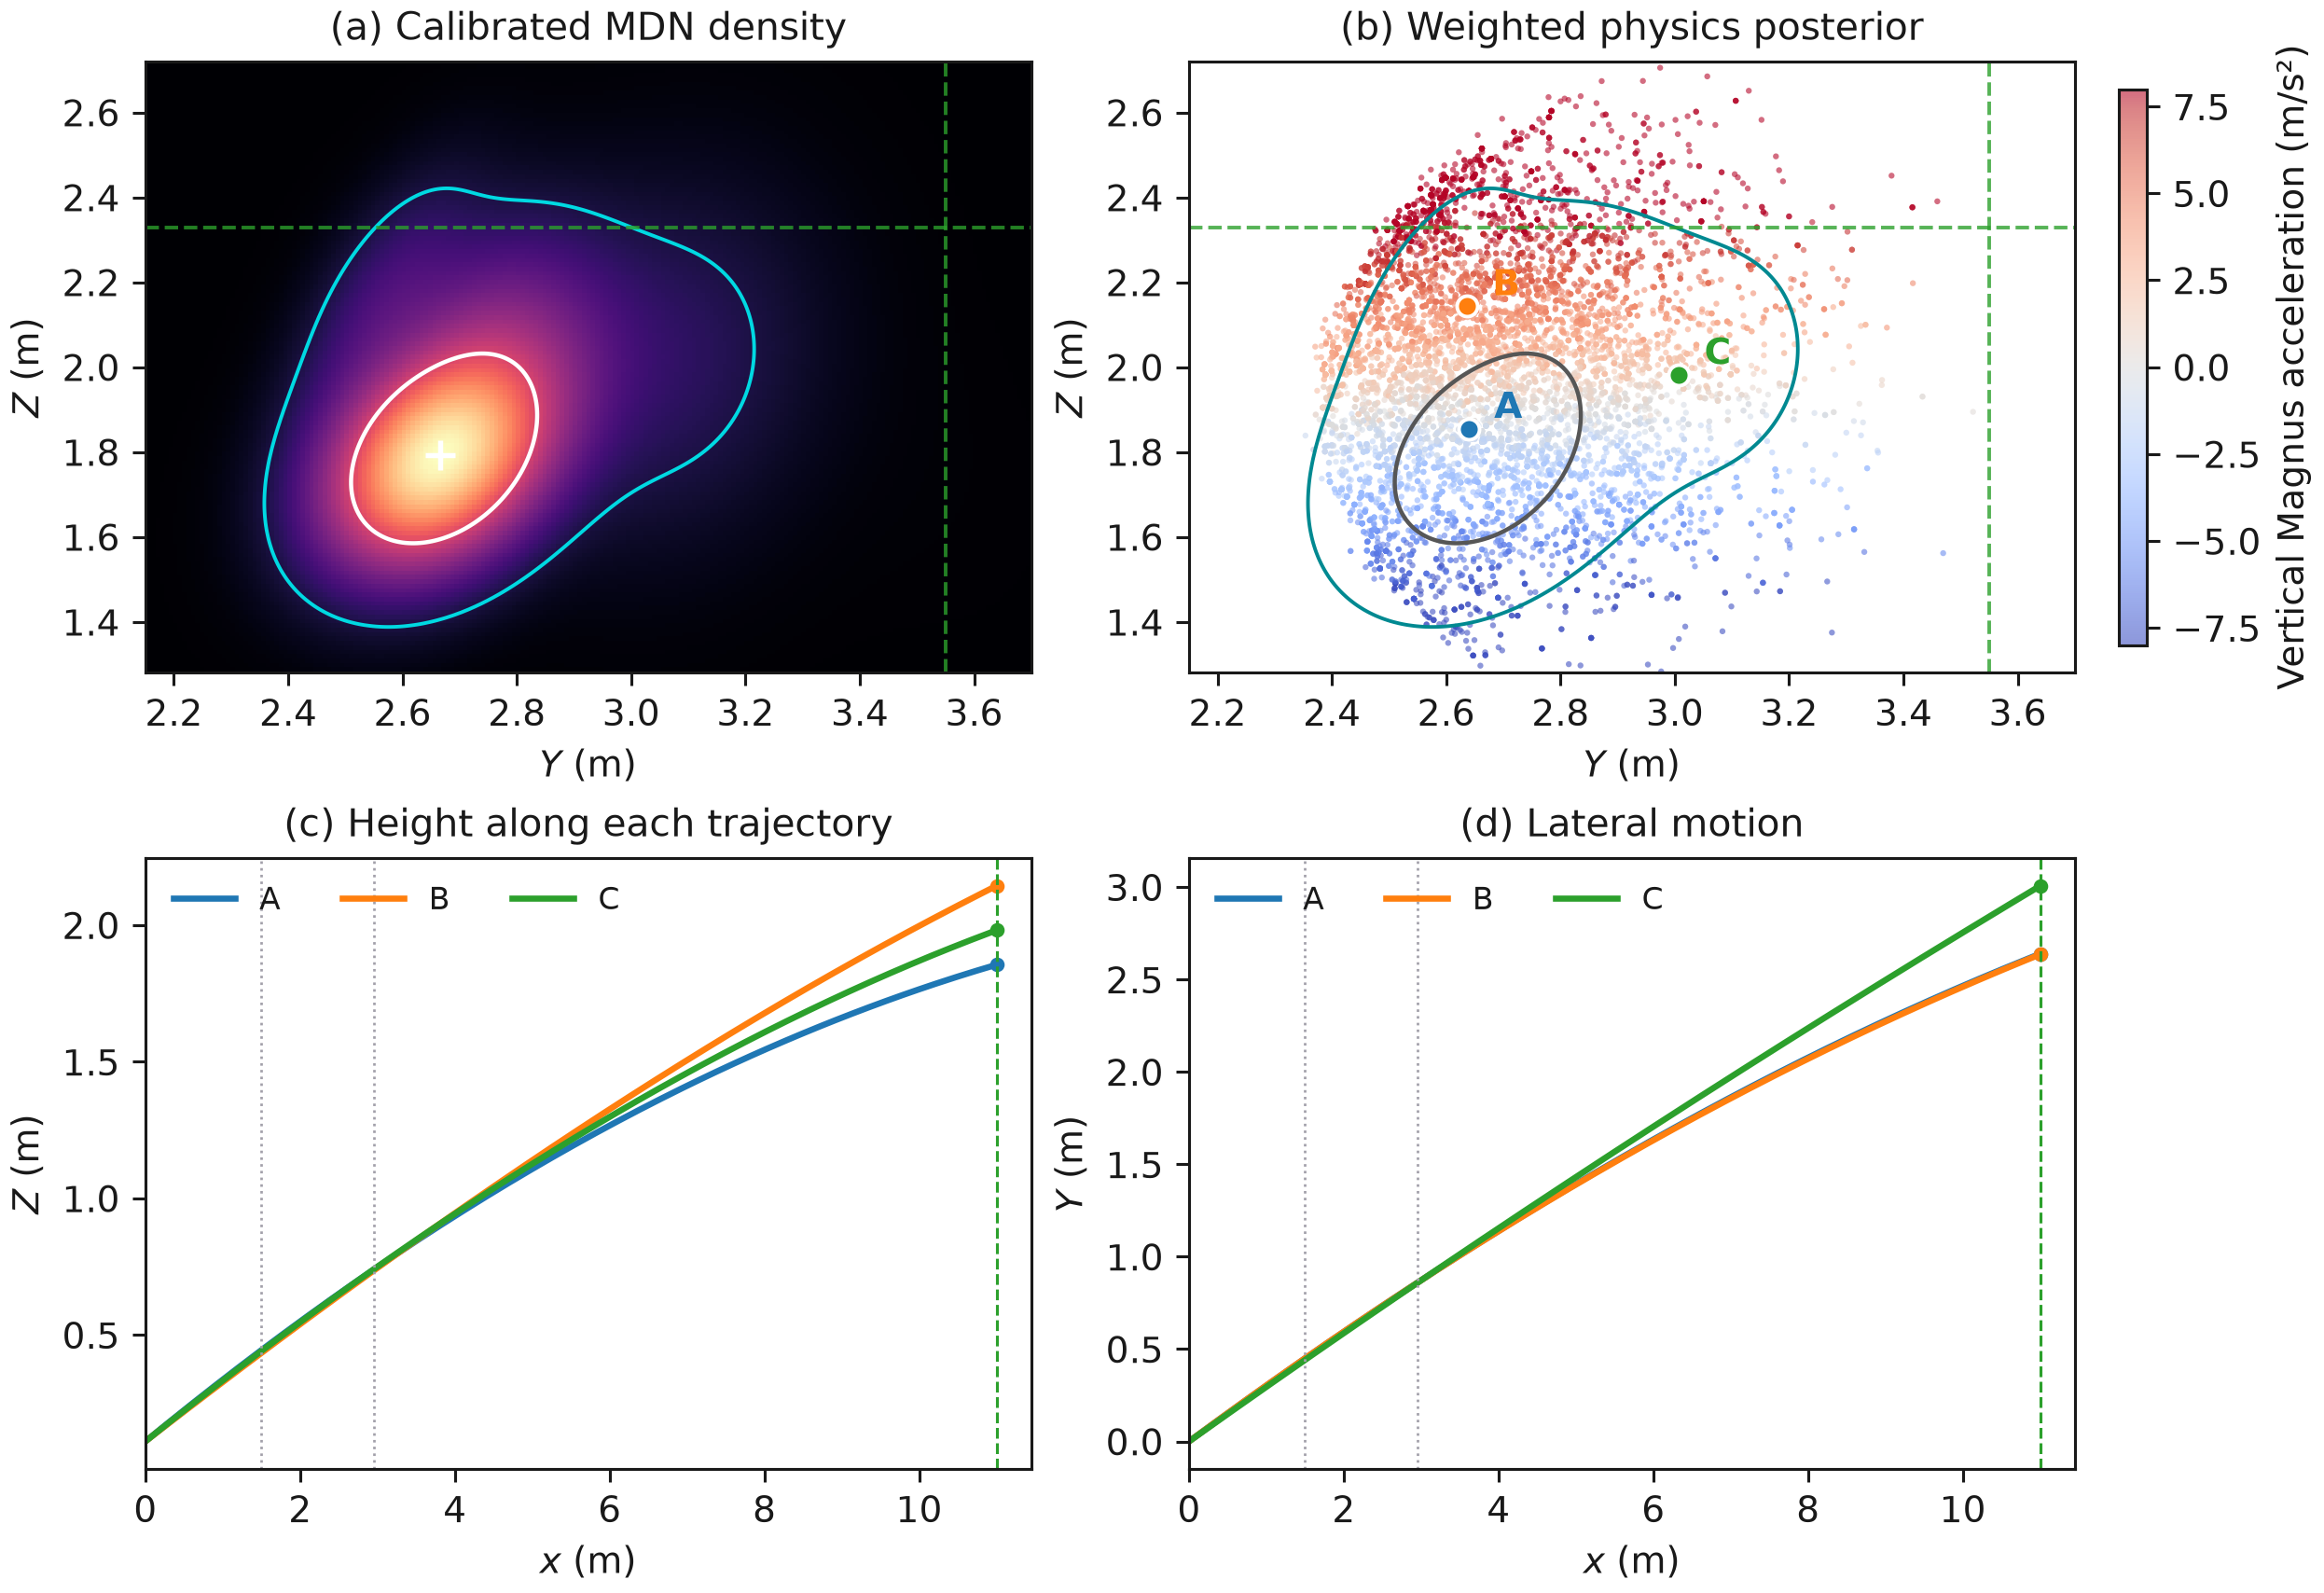
\includegraphics{assets/papers/two-points-to-the-goal/case_decomposition_v3.png}}
\caption{Fig. 2. Physical interpretation at $5\,\mathrm{mm}$. (a) Calibrated v3 density. (b) Weighted resamples from the physics posterior, coloured by vertical Magnus acceleration at the observed midpoint velocity, with the same v3 contours overlaid. (c, d) Representative trajectories. The dotted lines mark the observed longitudinal positions and the dashed green line marks the plane.}
\end{figure}

\begin{figure}

\href{assets/papers/two-points-to-the-goal/case_profiles_v3.png}{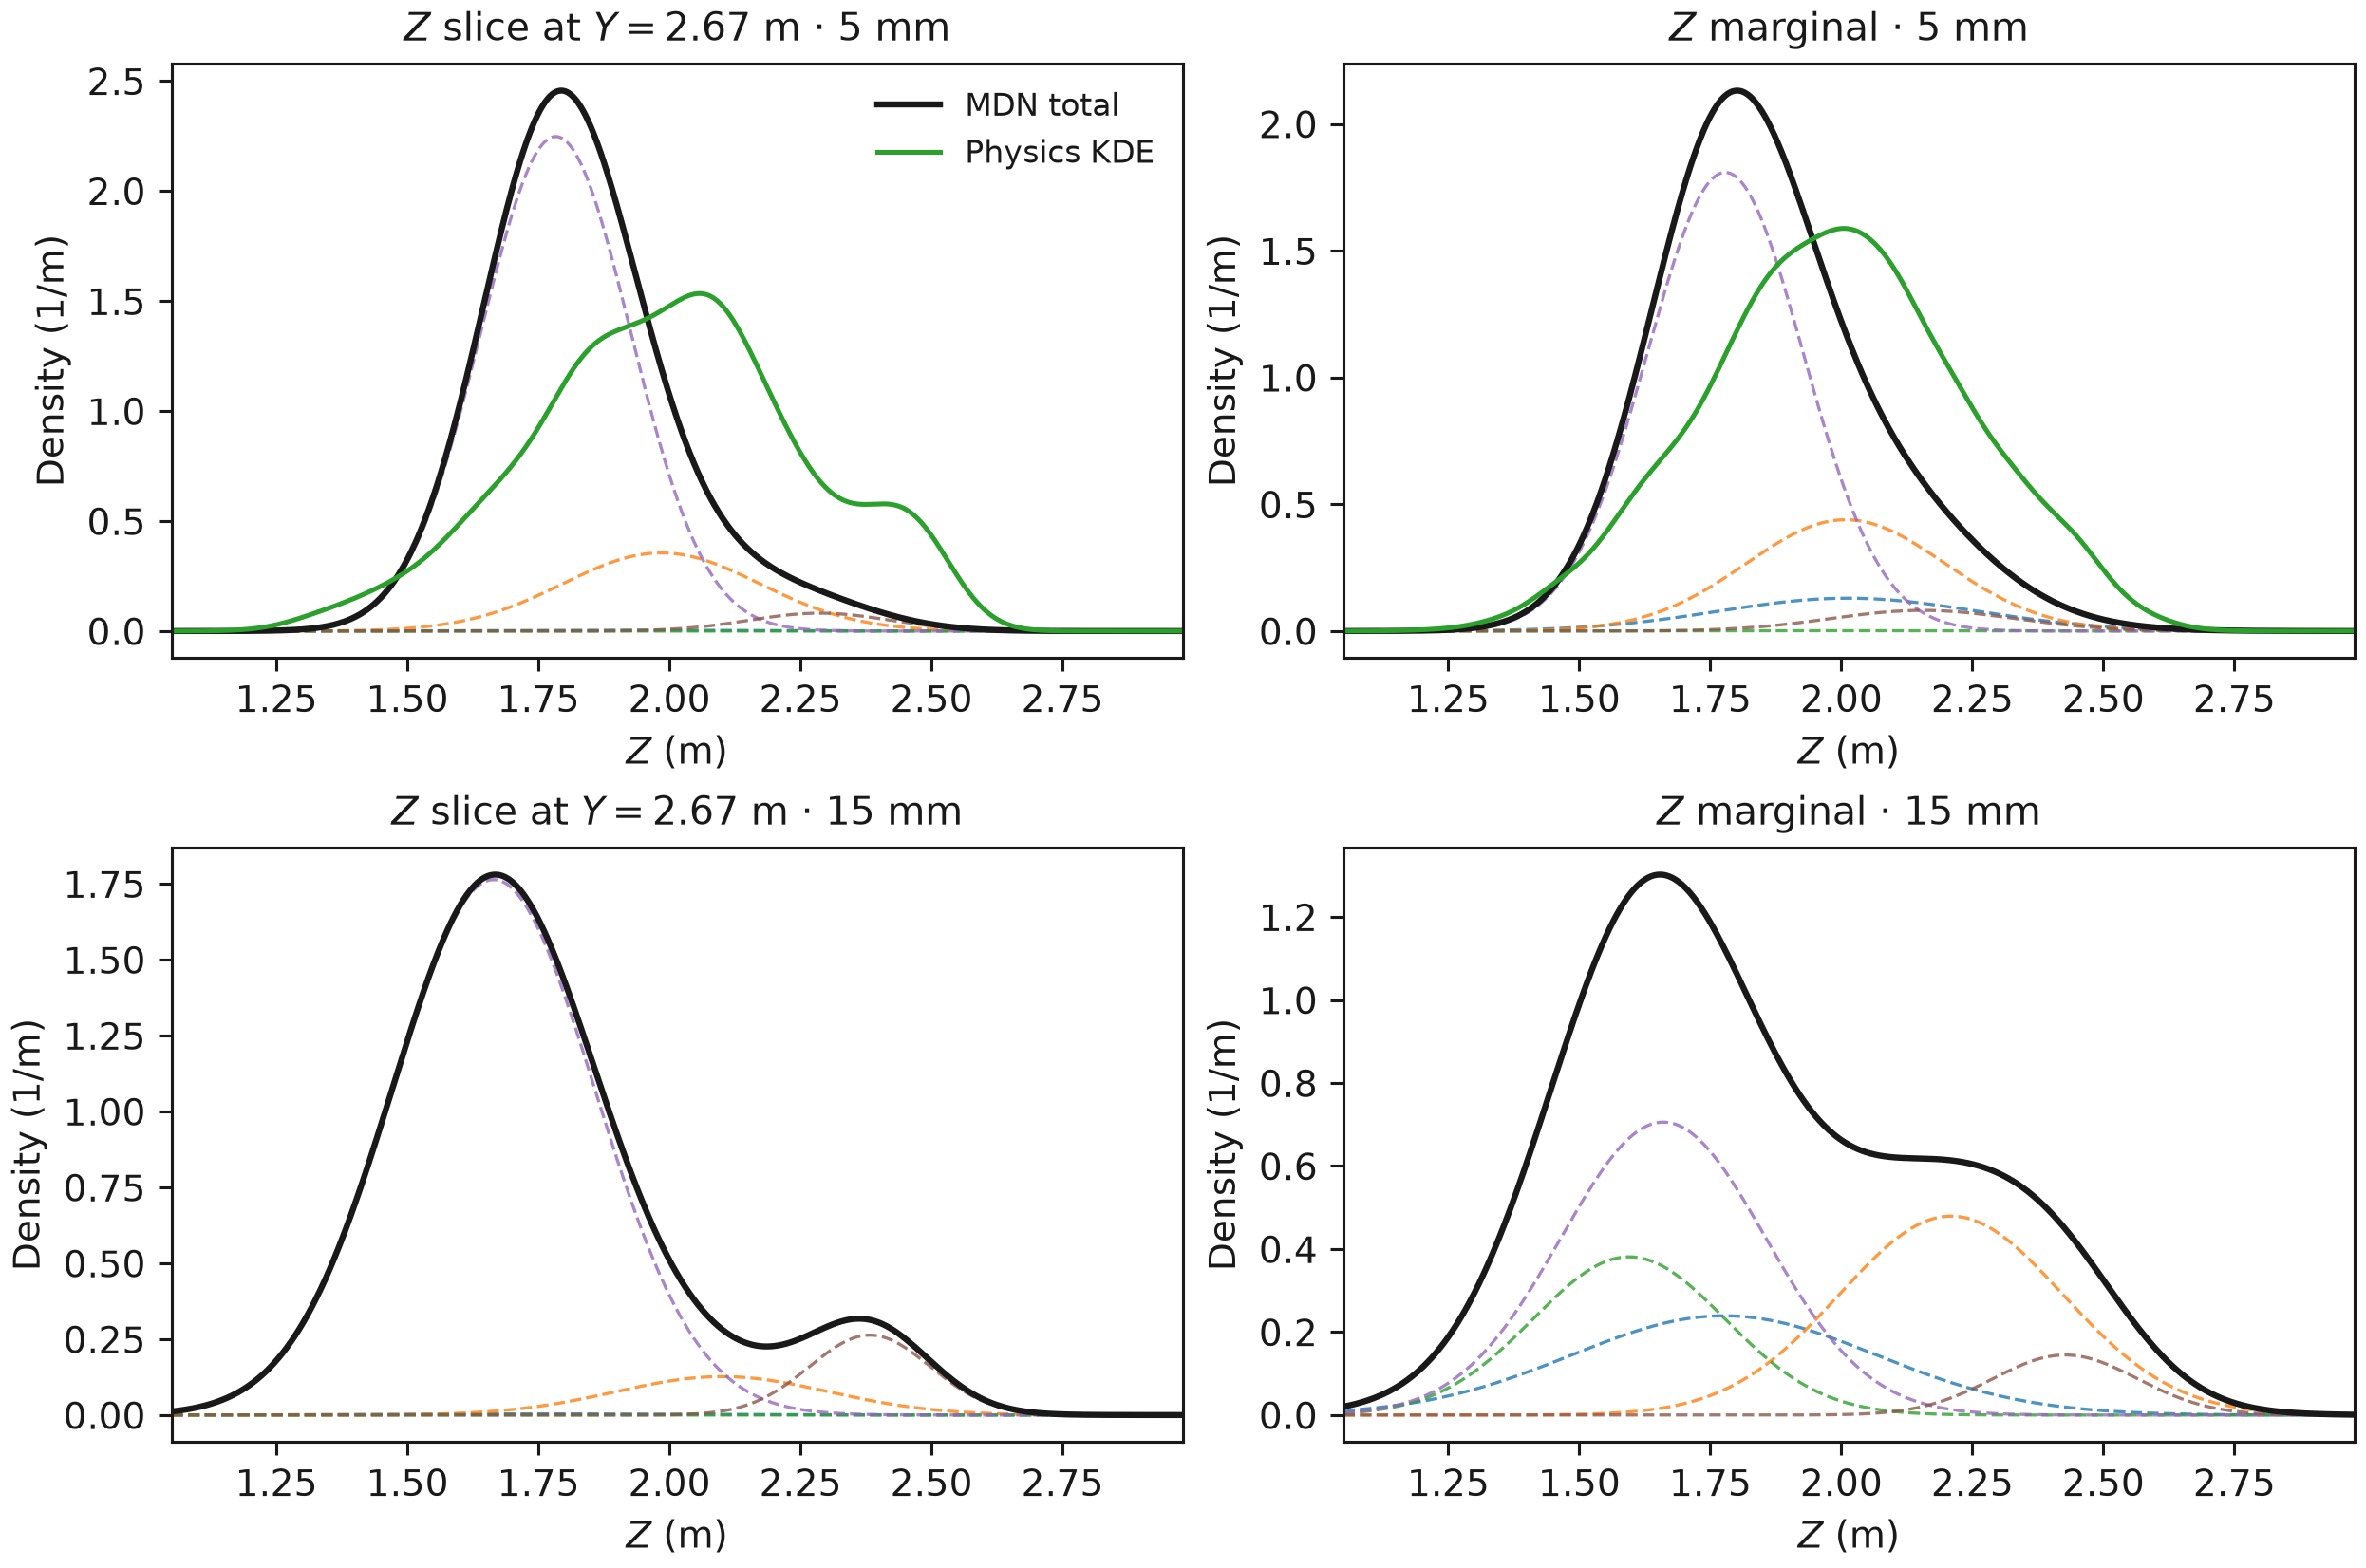
\includegraphics{assets/papers/two-points-to-the-goal/case_profiles_v3.png}}
\caption{Fig. 3. Seed-11 vertical slices and marginals. The dark solid curve is the total MDN density and dashed curves show its five weighted Gaussian components. Green shows the weighted physics KDE at $5\,\mathrm{mm}$ with Scott's bandwidth. The fixed-$Y$ slices are normalised to integrate to one over height.}
\end{figure}

\subsection{3.2 Feature, Target and Architecture Comparisons}

Physical features improve the direct model at $5\,\mathrm{mm}$ (C versus A in Table~5). The matched-budget Wiener model has the lowest mean test NLL among the retrained models at all four noise levels. Its median error at $5\,\mathrm{mm}$ is $0.269\,\mathrm{m}$, close to PI-ResMDN's $0.270\,\mathrm{m}$. Arm D reaches NLL $2.639$ at $15\,\mathrm{mm}$. The quadratic predictor has no finite forward root on $466$ of the $8{,}192$ test trajectories at this noise level, so D uses its zero-endpoint fallback on those rows.

\begin{table}[htbp]
  
  
  \caption{Table 5. Model comparison at $5\,\mathrm{mm}$ on the same $8{,}192$ v3 test trajectories and perturbations. Results average three seeds. Only the last row uses full training and calibration.}
  \begin{tabular}{lrrr}
    \toprule
    Model & Median (m) & P90 (m) & NLL \\
    \midrule
    Legacy coordinate MDN & 0.297 & 0.623 & $-0.073$ \\
    A: coordinates, direct & 0.282 & 0.603 & $-0.116$ \\
    B: coordinates, quadratic residual & 0.275 & 0.604 & $-0.140$ \\
    C: physics features, direct & 0.274 & 0.599 & $-0.173$ \\
    D: physics features, quadratic residual & 0.295 & 0.633 & $0.208$ \\
    E: coordinates + quadratic endpoint, residual & 0.274 & 0.607 & $-0.146$ \\
    PI-ResMDN, retrained & 0.270 & 0.598 & $-0.269$ \\
    Wiener-ResMDN, matched budget & 0.269 & 0.599 & $-0.300$ \\
    Wiener-ResMDN, full training and calibration & 0.266 & 0.597 & $-0.376$ \\
    \bottomrule
  \end{tabular}
\end{table}

In the two-layer SiLU screen, the 11- and 16-feature direct variants give selection NLLs of $-0.145$ and $-0.159$. Holding the Wiener input and residual target fixed, one, three and five mixture components give $-0.014$, $-0.186$ and $-0.238$. Four layers win the SiLU depth screen. At depth four, GELU gives the lowest mean NLL ($-0.253$), followed by Tanh ($-0.249$), SiLU ($-0.247$) and ReLU ($-0.222$), with variation across seeds (Fig.~4). This screen uses the smaller, matched training budget. At fixed GELU, the three- and four-layer models have nearly identical mean selection NLLs ($-0.2517$ and $-0.2532$, respectively), so we retain the original three-layer architecture.

In the three-layer GELU intervention screen, the reference mean selection NLL is $-0.252$. Removing within-component correlation, fixing the learning rate, and reusing one set of training perturbations per trajectory raise it to $-0.225$, $-0.208$ and $-0.168$, respectively.

\begin{figure}

\href{assets/papers/two-points-to-the-goal/architecture_v3.png}{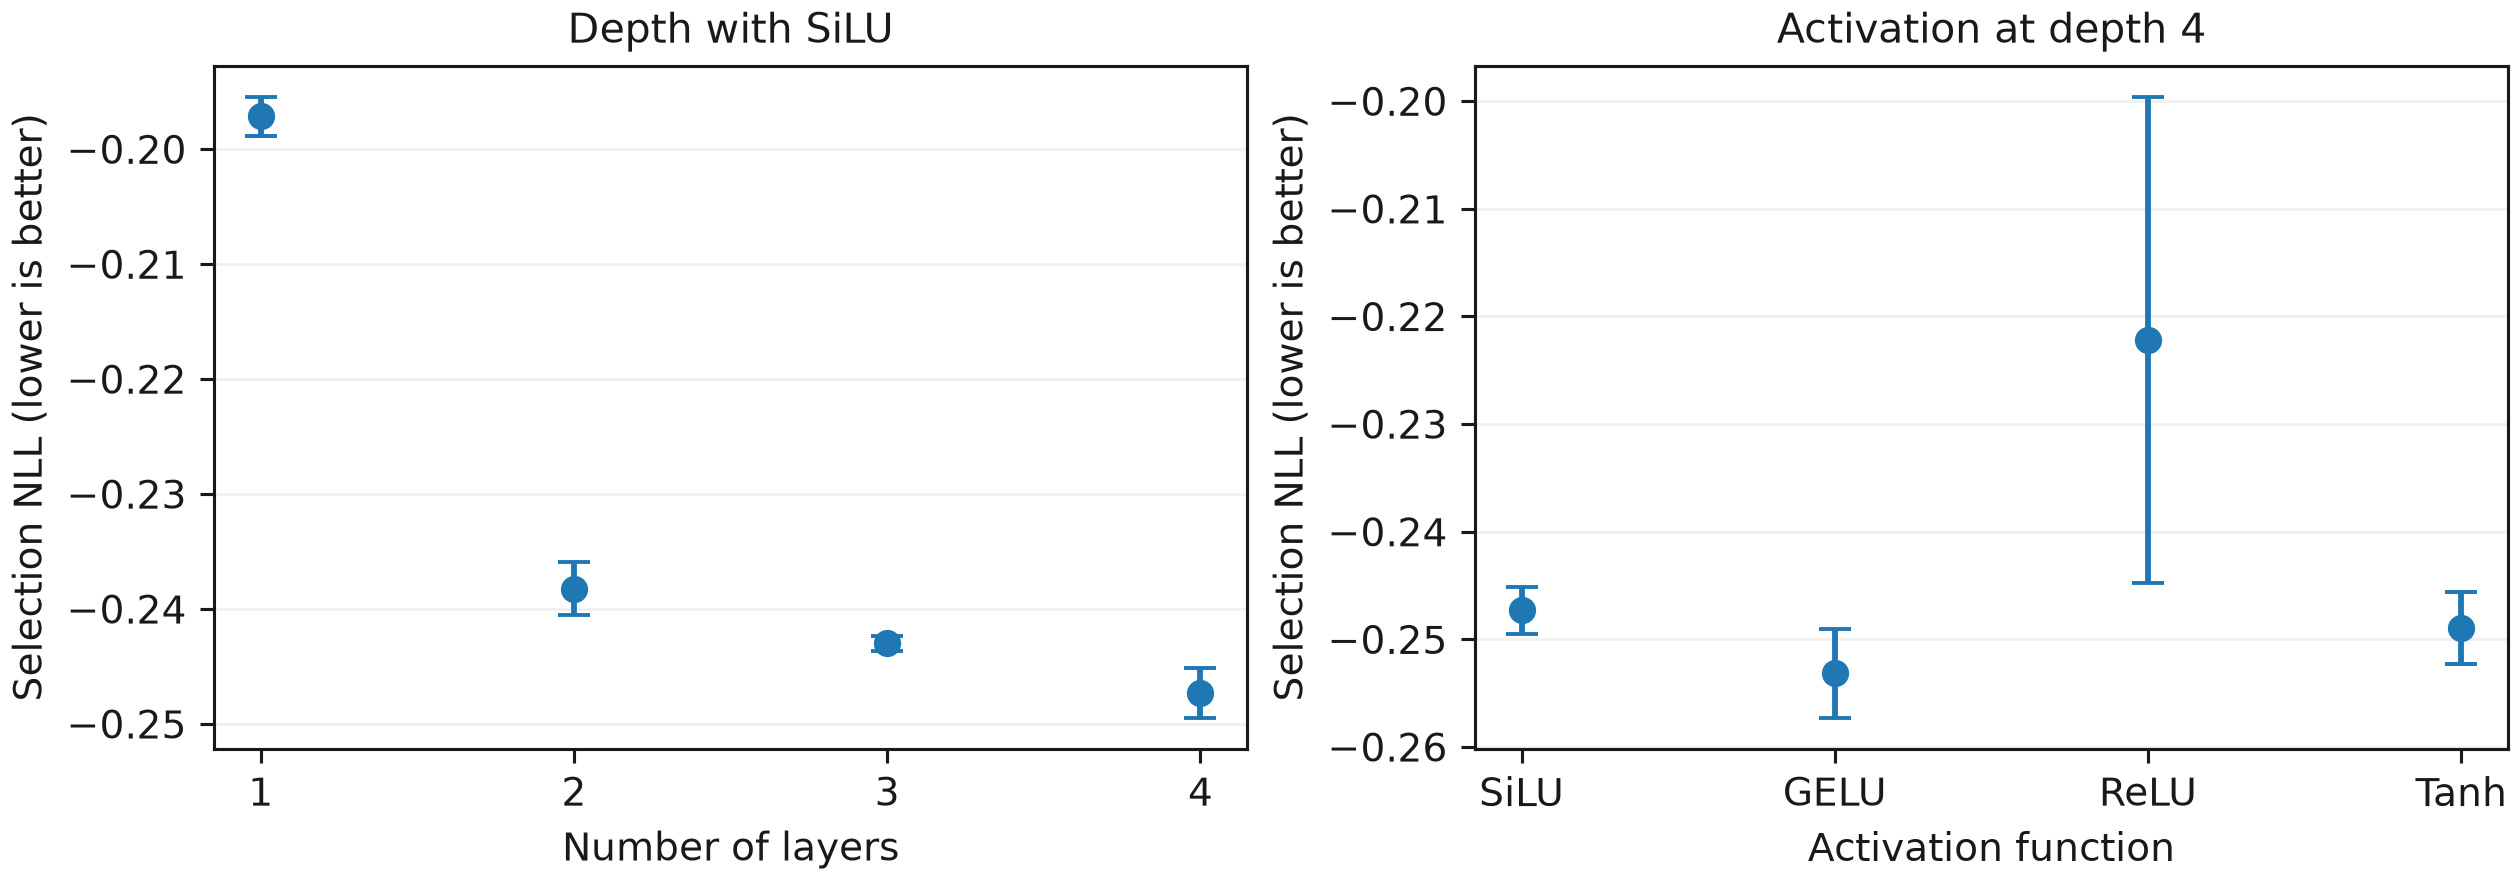
\includegraphics{assets/papers/two-points-to-the-goal/architecture_v3.png}}
\caption{Fig. 4. Depth and activation screens with the v3 Wiener residual inputs. Each point is the mean selection NLL across four noise levels and three training seeds. Error bars are sample standard deviations across seed means.}
\end{figure}

\subsection{3.3 Holdout Accuracy and Calibration}

Table~6 scores the $109{,}108$ held-out full-mixture crossings. At $5\,\mathrm{mm}$ the MDN median error is $0.266\,\mathrm{m}$ and the quadratic baseline's is $0.431\,\mathrm{m}$. The baseline uses identical coordinate perturbations and its error is computed on the subset with a finite forward root. The counts without a finite forward root are 0, 102, $2{,}139$ and $6{,}003$ at the four noise levels. The MDN produces a density for every test prefix.

\begin{table}[htbp]
  
  
  \caption{Table 6. Full-mixture v3 test results. Calibrated MDN scores are means over three training seeds. Point errors are in metres. HDR coverage is in percent.}
  \begin{tabular}{rrrrrrr}
    \toprule
    Noise (mm) & Quad.\ median & MDN median & MDN P90 & MDN NLL & $50\%$ HDR & $95\%$ HDR \\
    \midrule
    2  & 0.188 & 0.126 & 0.292 & $-1.766$ & 50.16 & 95.27 \\
    5  & 0.431 & 0.266 & 0.597 & $-0.371$ & 50.08 & 95.08 \\
    10 & 0.843 & 0.416 & 0.802 & $ 0.332$ & 50.58 & 95.32 \\
    15 & 1.235 & 0.488 & 0.868 & $ 0.590$ & 50.44 & 95.42 \\
    \bottomrule
  \end{tabular}
\end{table}

Table~7 and Fig.~5 separate scale fitting from HDR rank adjustment. Scale fitting changes coverage by at most $0.14$ percentage points. At $15\,\mathrm{mm}$, the full calibration raises inner coverage from $49.33\%$ to $50.44\%$ and lowers outer coverage from $95.87\%$ to $95.42\%$. The corresponding outer median area, averaged across seeds, drops from $2.018$ to $1.975\,\mathrm{m^2}$.

\begin{table}[htbp]
  
  
  \caption{Table 7. Calibration stages on the full test split. Coverage entries give the $50\%$ / $95\%$ regions in percent. The last column gives calibrated median areas in $\mathrm{m^2}$. All entries are averaged across seeds.}
  \begin{tabular}{rrrrr}
    \toprule
    Noise (mm) & Raw coverage & Scale only & Scale + HDR & Final areas \\
    \midrule
    2 & 50.15 / 95.22 & 50.29 / 95.27 & 50.16 / 95.27 & 0.040 / 0.201 \\
    5 & 49.77 / 95.44 & 49.81 / 95.45 & 50.08 / 95.08 & 0.171 / 0.854 \\
    10 & 49.71 / 95.74 & 49.65 / 95.72 & 50.58 / 95.32 & 0.375 / 1.659 \\
    15 & 49.33 / 95.87 & 49.26 / 95.84 & 50.44 / 95.42 & 0.497 / 1.975 \\
    \bottomrule
  \end{tabular}
\end{table}

Conditional in-frame expected calibration errors are $0.0032$, $0.0039$, $0.0044$ and $0.0056$ in increasing noise order. The Brier scores are $0.0226$, $0.0451$, $0.0644$ and $0.0731$. The observed in-frame fraction among simulated airborne crossings is $56.5\%$.

\begin{figure}

\href{assets/papers/two-points-to-the-goal/coverage_v3.png}{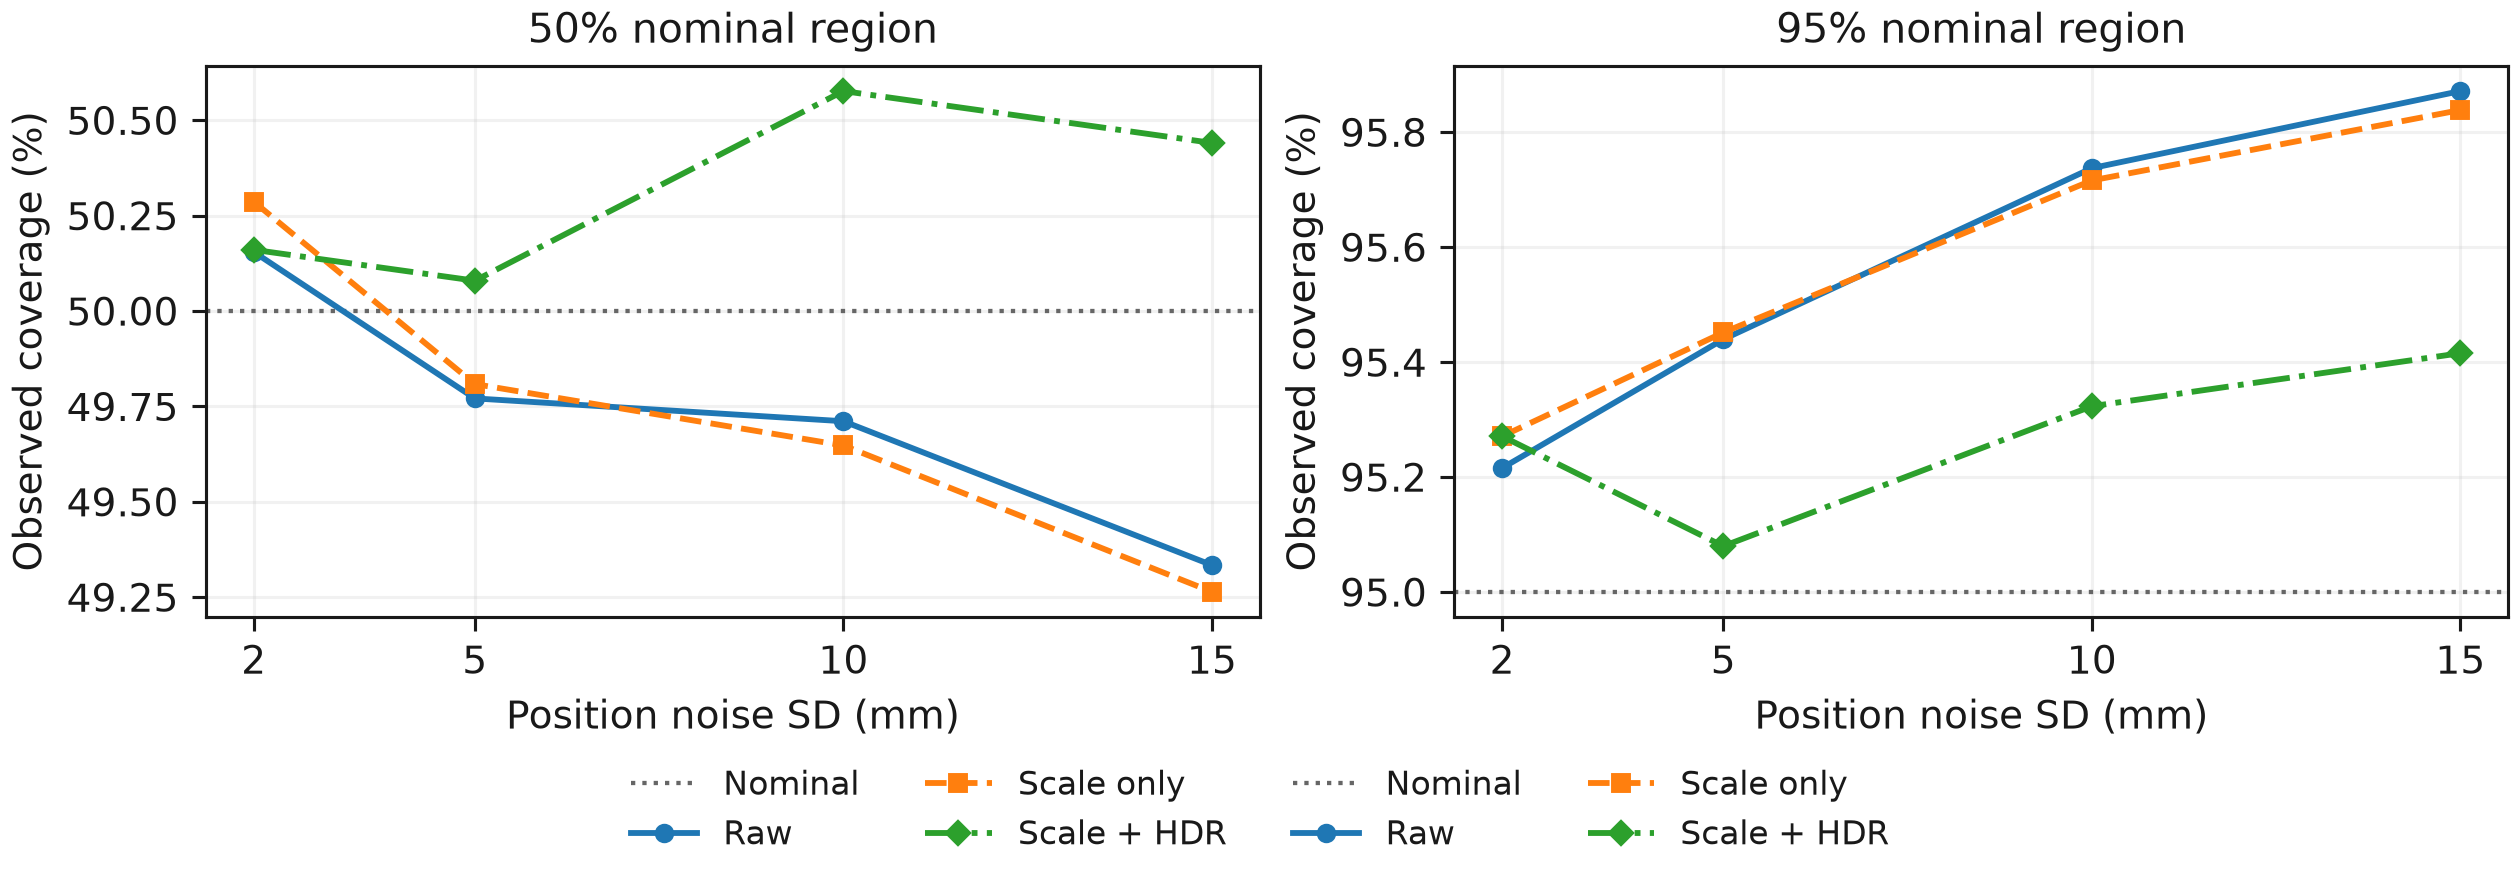
\includegraphics{assets/papers/two-points-to-the-goal/coverage_v3.png}}
\caption{Fig. 5. Observed joint-region coverage before calibration, after scale fitting, and after HDR rank adjustment on $109{,}108$ held-out v3 trajectories. The dotted lines give the nominal levels.}
\end{figure}

\subsection{3.4 Paired Comparison with the Physics Posterior}

We draw 32 trajectories from the v3 test split (seed 155108) and use the same $5\,\mathrm{mm}$ perturbation for each method. Adaptive importance sampling starts with $6{,}000$ proposals per stage and retries with $18{,}000$ when conditional ESS falls below 100. After retry, 30 trajectories meet the ESS threshold and have a finite quadratic prediction. The median Euclidean errors are $0.478\,\mathrm{m}$ for quadratic extrapolation, $0.314\,\mathrm{m}$ for the Bayesian reference and $0.270\,\mathrm{m}$ for the calibrated v3 model (seed 11).

Median energy scores are $0.241$ and $0.173$ for the Bayesian reference and v3 model, respectively. The energy score is $\mathbb E\|\mathbf Q-\mathbf q\|-\tfrac12\mathbb E\|\mathbf Q-\mathbf Q'\|$, with independent predictive draws $\mathbf Q,\mathbf Q'$ and truth $\mathbf q$ [25]. Median elapsed times on the same CPU are $2.19\,\mathrm{s}$ and $1.74\,\mathrm{ms}$, including inference, sampling or resampling $4{,}096$ endpoints, and scoring. The small ESS-filtered subset and the different prior distributions limit the accuracy comparison.

\subsection{3.5 Aimed Sampling and Asai Source Holdout}

With Asai withheld, aiming increases the count of airborne endpoints with $v_x\ge24\,\mathrm{m\,s^{-1}}$ within the sampling grid from $483{,}698$ to $550{,}313$ ($13.8\%$). The grid spans $|Y|\le3.66\,\mathrm{m}$ and $R\le Z\le2.44\,\mathrm{m}$ in $6\times3$ cells. Its least populated cell grows from $20{,}207$ to $24{,}984$. This design diagnostic uses the full lateral width and crossbar height.

On $53{,}126$ identical uniform-prior test trajectories with matched $5\,\mathrm{mm}$ perturbations, median error changes from $30.26$ to $30.09\,\mathrm{cm}$, while NLL changes from $-0.2602$ to $-0.2577$. Aiming changes both the distribution and the number of usable training trajectories. The comparison estimates their combined effect.

The Asai free kicks were tracked at $100\,\mathrm{Hz}$ with the goal at $23\,\mathrm{m}$ [5]. We take positions at $0.05$ and $0.10\,\mathrm{s}$ relative to the initial frame, shift the starting height to $R$ for inference, then restore the height offset and score against an interpolated crossing at a virtual $11\,\mathrm{m}$ plane. Table~8 uses the two models whose priors exclude these trials. It uses an assumed $\sigma=10\,\mathrm{mm}$ and the original measured positions. The full-mixture model uses the same kicks as prior anchors, so the source-holdout results apply to the two reduced mixtures.

\begin{table}[htbp]
  
  
  \caption{Table 8. Asai source holdout. Euclidean errors of the predictive mean, in centimetres, averaged over three training seeds.}
  \begin{tabular}{lrrrr}
    \toprule
    Sampling strategy & Fig3 & Sample05 & Sample12 & Mean over kicks \\
    \midrule
    \texttt{v2\_no\_asai} & 56.53 & 56.73 & 61.73 & 58.33 \\
    \texttt{v3\_no\_asai} & 57.59 & 57.51 & 62.28 & 59.13 \\
    \bottomrule
  \end{tabular}
\end{table}

The three observed kicks show no transfer gain from aiming under this noise assumption. The trial count and use of a virtual crossing plane limit the scope of the comparison.

\subsection{3.6 Distribution Shift}

We take $6{,}000$ v3 test launches (seed 155107), retain paired airborne crossings under each perturbation, and reuse the same $5\,\mathrm{mm}$ noise. With the seed-11 model and calibrator fixed, a $3\,\mathrm{m\,s^{-1}}$ crosswind ($5{,}978$ pairs) lowers $50\%$ coverage from $50.3\%$ to $42.8\%$ and $95\%$ coverage from $95.2\%$ to $91.9\%$. Spin decay with a $0.5\,\mathrm{s}$ time constant ($5{,}971$ pairs) lowers inner coverage from $50.7\%$ to $38.6\%$ while median error falls from $0.265$ to $0.234\,\mathrm{m}$. Smaller point error can coincide with worse coverage.

\subsection{3.7 Rebound and Rolling Crossings}

For low shots, we continue the flight when the ball centre reaches $z=R$. The vertical velocity reverses with normal restitution $e_n=0.60$. At impact, the horizontal slip is $\mathbf v_t+(\boldsymbol\omega\times(-R\hat{\mathbf z}))_t$. With thin-shell inertia $I=2mR^2/3$, the tangential impulse opposes slip and is capped at $\mu_c$ times the normal impulse ($\mu_c=0.40$). The impulse changes both horizontal velocity and spin. When the incoming normal speed drops below $0.50\,\mathrm{m\,s^{-1}}$, the ball rolls with resistance $\mu_r g$ ($\mu_r=0.08$) and quadratic drag. We extend the integration horizon to $3\,\mathrm{s}$. These coefficients define the simulated surface.

We use a separate $100{,}000$-launch v3 bank with the full anchor mixture. The simulator preserves the $88{,}999$ direct crossings and recovers $11{,}001$ additional crossings ($6{,}636$ during a rebound and $4{,}365$ while rolling). Of the post-contact crossings, $7{,}761$ are in-frame under the radius-inset criterion. The contact simulator supplies missing positions after impact, completing the 951 observation prefixes left incomplete by the airborne integrator. Varying $e_n$ over $0.56$--$0.67$, $\mu_c$ over $0.25$--$0.55$ and $\mu_r$ over $0.046$--$0.153$ one at a time leaves $11{,}001$ post-contact crossings in each simulated scenario. The in-frame count ranges from $7{,}742$ to $7{,}761$.

Two Wiener residual MDNs have the same architecture as Section~2.6, seed 11 and 100 training epochs. The airborne-only model trains on $71{,}202$ direct crossings. The contact-inclusive model trains on the same rows plus $8{,}798$ post-contact crossings. Each model uses its own selection and calibration folds from the same partition. Both are evaluated on the same $10{,}000$ rows with identical noise and receive only the two positions and $\sigma$ through the feature extractor. Ground-contact status defines evaluation subsets. The contact-inclusive model estimates the endpoint density conditional on crossing by either route.

\begin{table}[htbp]
  
  
  \caption{Table 9. Paired rebound experiment at $\sigma=5\,\mathrm{mm}$. In each cell, the first number is the airborne-only model and the second is the contact-inclusive model. Coverage is in percent.}
  \begin{tabular}{lrrrr}
    \toprule
    Test subset & Median (m) & NLL & $50\%$ HDR & $95\%$ HDR \\
    \midrule
    Direct ($n=8{,}899$) & 0.271 / 0.272 & $-0.288$ / $-0.268$ & 49.7 / 49.0 & 95.1 / 94.7 \\
    Post-contact ($n=1{,}101$) & 0.242 / 0.163 & $+0.053$ / $-3.181$ & 30.8 / 58.9 & 84.1 / 97.5 \\
    All ($n=10{,}000$) & 0.267 / 0.261 & $-0.251$ / $-0.588$ & 47.6 / 50.2 & 94.0 / 95.3 \\
    \bottomrule
  \end{tabular}
\end{table}

At $5\,\mathrm{mm}$, a paired row bootstrap gives a post-contact median error difference of $-0.080\,\mathrm{m}$ (95\% interval $[-0.089,-0.069]\,\mathrm{m}$) for contact-inclusive minus airborne-only training. The direct-crossing difference is $+0.001\,\mathrm{m}$ ($[-0.001,+0.003]\,\mathrm{m}$). The post-contact $50\%$ region still overcovers at $58.9\%$, and $22.0\%$ of its predictive samples lie below $Z=R$ because the Gaussian mixture is untruncated. A 200-epoch airborne-only control gives a post-contact median error of $0.244\,\mathrm{m}$ and outer coverage of $80.3\%$ at the same noise.

For the stated kick, the two models give modes of $(2.661,1.798)$ and $(2.655,1.793)\,\mathrm{m}$ at $5\,\mathrm{mm}$. A separate importance-sampling audit with the uniform reference prior assigns numerically negligible mass to first contact before crossing. At $5\,\mathrm{mm}$ the two runs have ESS $2{,}132$ and $1{,}767$. These finite samples support treating the case as a direct crossing in this model. They provide no quantitative upper bound on the rare-event probability.

\subsection{3.8 Sensitivity to the Drag Prior}

For the stated kick, raising the upper bound of $C_D$ from $0.30$ to $0.45$ shifts the posterior mean by about $2\,\mathrm{cm}$. Mean $50\%$ and $95\%$ areas change by $+1.1\%$ and $-0.5\%$, respectively, less than the variation across the three seeds.

\begin{table}[htbp]
  
  \caption{Table 10. Sensitivity of the case posterior to the upper limit of the drag prior ($\sigma=5\,\mathrm{mm}$, three seeds, $40{,}000$ samples per stage). Ranges are minima and maxima over seeds; means are averages over seeds.}
  \begin{tabular}{lccc}
    \toprule
    $C_D$ prior & $50\%$ area ($\mathrm{m^2}$) & $95\%$ area ($\mathrm{m^2}$) & Mean $(Y,Z)$ (m) \\
    \midrule
    $U[0.15,0.30]$ & 0.213 (0.205--0.219) & 0.806 (0.789--0.821) & (2.70, 1.99) \\
    $U[0.15,0.45]$ & 0.215 (0.210--0.222) & 0.802 (0.792--0.809) & (2.69, 1.97) \\
    \bottomrule
  \end{tabular}
\end{table}

\subsection{3.9 Model-Form Check on Tracked Arcs}

We fit the first six frames of ISSIA-3D segments 608--622 and 1144--1172, sampled at $25\,\mathrm{fps}$, and score the remaining frames [15, 16]. Selection required at least two cameras, eight consecutive frames, height of at least $0.30\,\mathrm{m}$ and median reprojection error below $10$ pixels per frame. Absolute 3D accuracy and action labels were unverified for these segments.

Drag reduces held-out RMSE in both arcs. Adding an effective lift component in the vertical plane gives the lowest errors (Table~11). The fitted drag and lift have large uncertainties and may absorb tracking or model error. These suffix forecasts check the flight equations. Related ISSIA arcs and the DFL penalties below also contribute to the main simulation prior.

\begin{table}[htbp]
  
  \caption{Table 11. Held-out RMSE and last-frame error, in metres, for two ISSIA arcs. Initial conditions and any free aerodynamic coefficients use the first six frames.}
  \begin{tabular}{llcccc}
    \toprule
    Arc & Quantity & Gravity & $C_D=0.22$ & $C_D=0.45$ & Drag + lift \\
    \midrule
    608--622 & Forecast RMSE & 0.697 & 0.489 & 0.469 & \textbf{0.188} \\
             & Final error   & 1.243 & 0.863 & 0.811 & \textbf{0.308} \\
    1144--1172 & Forecast RMSE & 2.179 & 1.546 & 1.584 & \textbf{1.084} \\
               & Final error   & 4.169 & 2.876 & 2.942 & \textbf{2.119} \\
    \bottomrule
  \end{tabular}
\end{table}

\subsection{3.10 Prefix Forecasts on Tracked Flights}

We fit the first three DFL positions at $0$, $0.04$ and $0.08\,\mathrm{s}$ and forecast the held-out trajectory in local coordinates [17]. Both kicks resulted in goals. The start frames are 128955 and 176244 (events 18232100000995 and 18242100001386). With $15\,\mathrm{mm}$ assumed noise, unknown spin improves one crossing estimate and slightly worsens the other (Table~12).

Unknown spin raises held-out RMSE from $0.338$ to $0.366\,\mathrm{m}$ on ISSIA frames 2972--2991. For 22 held-out planar positions digitised from Barber and Carr\'e's Fig.~5, RMSE rises from $2.266$ to $2.301\,\mathrm{m}$ at an assumed $67\,\mathrm{mm}$ digitisation scale [18].

\begin{table}[htbp]
  
  \caption{Table 12. Two DFL penalties with seven scored positions before each reference crossing. Both trajectory RMSE and crossing-point error are in metres. The crossing forecasts condition on airborne arrival at each observed goal plane.}
  \begin{tabular}{lrrrr}
    \toprule
    & \multicolumn{2}{c}{Trajectory RMSE} & \multicolumn{2}{c}{Crossing error} \\
    \cmidrule(lr){2-3}\cmidrule(lr){4-5}
    Case & Zero spin & Unknown spin & Zero spin & Unknown spin \\
    \midrule
    J03WOH & 0.347 & 0.292 & 0.645 & 0.543 \\
    J03WR9 & 0.309 & 0.305 & 0.542 & 0.553 \\
    \bottomrule
  \end{tabular}
\end{table}

Of 60 DFL flight candidates, 11 passed motion and event screening. At both $15$ and $30\,\mathrm{mm}$, unknown spin lowers held-out RMSE in 7 of 11 segments, with median paired improvements of $0.027$ and $0.011\,\mathrm{m}$. The screen fits a quadratic to the full segment, including later frames, and favours smooth arcs. These segments lack goal-plane labels.

\section{4 Discussion}

Two noisy positions constrain average velocity more tightly than acceleration. The Wiener anchor shrinks the quadratic estimate more strongly as $\sigma$ increases, while the mixture learns corrections and can represent several plausible crossing locations. The neural network provides a predictive density in a single forward pass. The wind and spin-decay tests show how forecast coverage deteriorates when the flight dynamics depart from the training model.

Aiming increases sampling density in the high-speed target grid. The shared uniform-prior test shows a small decrease in median point error and a small increase in NLL. The three source-held-out Asai replays use reduced mixtures and an assumed measurement noise. The DFL and ISSIA checks address individual physical trajectories, including trajectories used to construct the full-mixture prior. Calibration for real penalties remains unmeasured. The earlier v1 results use a uniform test distribution and a ball-centre goal rectangle. Comparison with v3 calls for shared test flights, noise and goal geometry.

The airborne model forecasts geometric in-frame arrival conditional on $\mathcal E$. The contact-inclusive model conditions on crossing by either route within the simulated horizon. An unconditional in-frame forecast requires a separate estimate of crossing probability. The geometry accounts for ball radius and omits frame contact and goalkeeper intervention. The post-contact comparison uses one training seed and depends on the assumed surface parameters and simulated mix of rebounds and rolls. The untruncated mixture assigns $22.0\%$ of post-contact draws to heights below one ball radius. A physically constrained density would require recalibration and fresh coverage checks. Estimating the probabilities of direct crossing, post-contact crossing and failure to reach the plane remains a separate task. External validation requires holding out entire matches or data sources and including shots that miss or touch the ground.

In a local calculation on held-out v3 launches, an additional $0.15\,\mathrm{s}$ observation with the same $5\,\mathrm{mm}$ noise reduces the median radial crossing spread from $0.284$ to $0.112\,\mathrm{m}$ under a Gaussian reference prior (Appendix~A.3). This measurement design adds $50\,\mathrm{ms}$ before the forecast can be made.

An interactive demonstration (\url{https://navi.x1shang.top/learning/penalty/}) runs the v3 predictor in the browser and lets readers vary the observations and assumed noise. It recomputes contours on its display grid, so region areas can differ slightly from the values reported here.

\section{5 Conclusion and Outlook}

At an assumed $5\,\mathrm{mm}$ coordinate noise, the million-trajectory MDN predicts a most likely crossing at $(2.67,1.79)\,\mathrm{m}$ for the stated kick. Its $95\%$ region covers $95.1\%$ of the held-out still-air simulations at this noise level. On tracked data, the source-held-out MDNs had mean crossing errors of $0.58$--$0.59\,\mathrm{m}$ over three Asai free kicks at a virtual $11\,\mathrm{m}$ plane with $10\,\mathrm{mm}$ assumed noise. Bayesian forecasts with unknown spin had crossing errors of $0.54$ and $0.55\,\mathrm{m}$ on two DFL penalties with $15\,\mathrm{mm}$ assumed noise. Coverage on real penalties remains unmeasured. Crosswind reduces coverage under the fixed model. In the single-seed paired experiment on the specified simulated surface, contact-inclusive training reduces the post-contact median error from $0.242$ to $0.163\,\mathrm{m}$, with a $1\,\mathrm{mm}$ median difference on direct crossings. The post-contact inner region covers $58.9\%$ and $22.0\%$ of its predictive draws fall below the physical height limit. High-rate tracking with independently measured noise and a real holdout spanning direct crossings, misses and ground contact would test these findings.

\begin{thebibliography}{99}

\addcontentsline{toc}{section}{References}

\bibitem{ifab} International Football Association Board, \emph{Laws of the Game 2025/26}, Laws 1 and 2 (field dimensions, penalty mark, ball). \url{https://www.theifab.com/laws/2025-26/the-field-of-play/} and \url{https://www.theifab.com/laws/2025-26/the-ball/}.
\bibitem{upc2026} University Physics Competition, \emph{2026 Problem B: Predicting FIFA Penalty Trajectories} (2026). \url{https://www.uphysicsc.com/2026contest.html}.
\bibitem{asai2007} T. Asai, K. Seo, O. Kobayashi, and R. Sakashita, “Fundamental aerodynamics of the soccer ball,” \emph{Sports Engineering} \textbf{10}(2), 101--109 (2007). \url{https://doi.org/10.1007/BF02844207}.
\bibitem{asai2013} T. Asai and K. Seo, “Aerodynamic drag of modern soccer balls,” \emph{SpringerPlus} \textbf{2}, 171 (2013). \url{https://doi.org/10.1186/2193-1801-2-171}.
\bibitem{asai2020} T. Asai, K. Kimachi, R. Liu, M. Koido, M. Nakayama, J. E. Goff, and S. Hong, “Measurements of the flight trajectory of a spinning soccer ball and the Magnus force acting on it,” \emph{Proceedings} \textbf{49}(1), 88 (2020). \url{https://www.mdpi.com/2504-3900/49/1/88}.
\bibitem{goff2010} J. E. Goff and M. J. Carr\'e, “Soccer ball lift coefficients via trajectory analysis,” \emph{European Journal of Physics} \textbf{31}(4), 775--784 (2010). \url{https://doi.org/10.1088/0143-0807/31/4/007}.
\bibitem{goff2017} J. E. Goff, J. Kelley, C. M. Hobson, K. Seo, T. Asai, and S. B. Choppin, “Creating drag and lift curves from soccer trajectories,” \emph{European Journal of Physics} \textbf{38}(4), 044003 (2017). \url{https://doi.org/10.1088/1361-6404/aa6fcd}.
\bibitem{bray2003} K. Bray and D. G. Kerwin, “Modelling the flight of a soccer ball in a direct free kick,” \emph{Journal of Sports Sciences} \textbf{21}(2), 75--85 (2003). \url{https://doi.org/10.1080/0264041031000070994}.
\bibitem{team358} Team 358, “The best strategy for penalty kicks,” University Physics Competition 2022, gold-medal paper, Section 3.1.4. \url{https://www.uphysicsc.com/2022-GM-B-358.pdf}.
\bibitem{nasaforces} NASA Glenn Research Center, “Forces on a soccer ball,” Beginner's Guide to Aeronautics. \url{https://www1.grc.nasa.gov/beginners-guide-to-aeronautics/forces-on-a-soccer-ball/}.
\bibitem{nasadrag} NASA Glenn Research Center, “Drag on a soccer ball,” Beginner's Guide to Aeronautics. \url{https://www1.grc.nasa.gov/beginners-guide-to-aeronautics/drag-on-a-soccer-ball/}.
\bibitem{nasalift} NASA Glenn Research Center, “Lift equation,” Beginner's Guide to Aeronautics. \url{https://www1.grc.nasa.gov/beginners-guide-to-aeronautics/lift-equation/}.
\bibitem{archimedes} NASA Glenn Research Center, “Buoyancy: Archimedes' principle,” Wind Tunnel Activities. \url{https://www.grc.nasa.gov/www/k-12/WindTunnel/Activities/buoy_Archimedes.html}.
\bibitem{loshchilov2019} I. Loshchilov and F. Hutter, “Decoupled weight decay regularization,” in \emph{Proceedings of the 7th International Conference on Learning Representations} (ICLR, 2019). \url{https://arxiv.org/abs/1711.05101}.
\bibitem{soccernetv3d} M. Guti\'errez-P\'erez and A. Agudo, “SoccerNet-v3D: Leveraging sports broadcast replays for 3D scene understanding,” in \emph{Proceedings of the IEEE/CVF Conference on Computer Vision and Pattern Recognition Workshops} (CVPRW, 2025), pp. 6024--6033; arXiv:2504.10106. \href{https://openaccess.thecvf.com/content/CVPR2025W/CVSPORTS/html/Gutierrez-Perez_SoccerNet-v3D_Leveraging_Sports_Broadcast_Replays_for_3D_Scene_Understanding_CVPRW_2025_paper.html}{CVF Open Access}.
\bibitem{issia} ISSIA-CNR, \emph{Soccer video sequences and annotations: download page} (acquisition description, 25 fps). Istituto di Studi sui Sistemi Intelligenti per l'Automazione, Consiglio Nazionale delle Ricerche. \url{https://pspagnolo.jimdofree.com/download/}.
\bibitem{dfl2025} M. Bassek, R. Rein, H. Weber, and D. Memmert, “An integrated dataset of spatiotemporal and event data in elite soccer,” \emph{Scientific Data} \textbf{12}, 195 (2025). \url{https://doi.org/10.1038/s41597-025-04505-y}; dataset: \url{https://doi.org/10.6084/m9.figshare.28196177}.
\bibitem{barber2010} S. Barber and M. J. Carr\'e, “The effect of surface geometry on soccer ball trajectories,” \emph{Sports Engineering} \textbf{13}(1), 47--55 (2010). \url{https://doi.org/10.1007/s12283-010-0048-x}.
\bibitem{bishop1994} C. M. Bishop, “Mixture density networks,” Technical Report NCRG/94/004, Aston University (1994). \url{https://www.microsoft.com/en-us/research/wp-content/uploads/2016/02/bishop-ncrg-94-004.pdf}.
\bibitem{gum2008} Joint Committee for Guides in Metrology, \emph{Evaluation of Measurement Data---Guide to the Expression of Uncertainty in Measurement}, JCGM 100:2008, Section 5.1.2. \url{https://doi.org/10.59161/JCGM100-2008E}.
\bibitem{layernorm2016} J. L. Ba, J. R. Kiros, and G. E. Hinton, “Layer normalization,” arXiv:1607.06450 (2016). \url{https://arxiv.org/abs/1607.06450}.
\bibitem{gelu2016} D. Hendrycks and K. Gimpel, “Gaussian error linear units (GELUs),” arXiv:1606.08415 (2016). \url{https://arxiv.org/abs/1606.08415}.
\bibitem{silu2018} S. Elfwing, E. Uchibe, and K. Doya, “Sigmoid-weighted linear units for neural network function approximation in reinforcement learning,” \emph{Neural Networks} \textbf{107}, 3--11 (2018). \url{https://doi.org/10.1016/j.neunet.2017.12.012}.
\bibitem{hyndman1996} R. J. Hyndman, “Computing and graphing highest density regions,” \emph{The American Statistician} \textbf{50}(2), 120--126 (1996). \url{https://doi.org/10.1080/00031305.1996.10474359}.
\bibitem{gneiting2007} T. Gneiting and A. E. Raftery, “Strictly proper scoring rules, prediction, and estimation,” \emph{Journal of the American Statistical Association} \textbf{102}(477), 359--378 (2007). \url{https://doi.org/10.1198/016214506000001437}.

\bibitem{hpdsplit2022} R. Izbicki, G. Shimizu, and R. B. Stern, \emph{CD-split and HPD-split: Efficient conformal regions in high dimensions}, \emph{Journal of Machine Learning Research} \textbf{23}(87), 1--32 (2022). \url{https://www.jmlr.org/papers/v23/20-797.html}.
\bibitem{harris2020} C. R. Harris et al., “Array programming with NumPy,” \emph{Nature} \textbf{585}, 357--362 (2020). \url{https://doi.org/10.1038/s41586-020-2649-2}.
\bibitem{virtanen2020} P. Virtanen et al., “SciPy 1.0: fundamental algorithms for scientific computing in Python,” \emph{Nature Methods} \textbf{17}, 261--272 (2020). \url{https://doi.org/10.1038/s41592-019-0686-2}.
\bibitem{paszke2019} A. Paszke et al., “PyTorch: An imperative style, high-performance deep learning library,” in \emph{Advances in Neural Information Processing Systems} \textbf{32}, 8024--8035 (2019). \href{https://proceedings.neurips.cc/paper_files/paper/2019/hash/bdbca288fee7f92f2bfa9f7012727740-Abstract.html}{NeurIPS proceedings}.
\bibitem{hunter2007} J. D. Hunter, “Matplotlib: A 2D graphics environment,” \emph{Computing in Science \& Engineering} \textbf{9}(3), 90--95 (2007). \url{https://doi.org/10.1109/MCSE.2007.55}.
\end{thebibliography}

\section*{Appendix A · Constant-Acceleration Baseline and Noise Propagation}

\subsection*{A.1 Baseline from the Three Given Positions}

For the three given positions and $\Delta t=0.05\,\mathrm{s}$, the midpoint velocity and acceleration are

$$
\begin{aligned}
\mathbf v(\Delta t)&=\frac{\mathbf r_2-\mathbf r_0}{2\Delta t}=(29.6,8.6,6.3)\,\mathrm{m\,s^{-1}},\\
  \mathbf a&=\frac{\mathbf r_2-2\mathbf r_1+\mathbf r_0}{\Delta t^2}=(-16,-16,-12)\,\mathrm{m\,s^{-2}}.
\end{aligned}
$$

Writing $\tau=T-\Delta t$, solve $-8\tau^2+29.6\tau-9.5=0$ and take the earlier forward root, $\tau=0.355\,\mathrm{s}$. Substitution gives $T=0.405\,\mathrm{s}$ and

$$
(Y,Z)=(0.45+8.6\tau-8\tau^2,\;0.44+6.3\tau-6\tau^2)=(2.495,1.920)\,\mathrm{m}.
$$

The benchmark baseline selects the earliest finite quadratic root after $0.10\,\mathrm{s}$, with a linear branch when $a_x$ is near zero.

\subsection*{A.2 Propagation of Position Noise to the Endpoint}

With an exact start and two independent coordinate errors of variance $\sigma^2$, the second difference has error $\boldsymbol\varepsilon_2-2\boldsymbol\varepsilon_1$ and component variance $5\sigma^2$ [20]. Thus

$$
\sigma_a=\frac{\sqrt{5}\,\sigma}{\Delta t^2}=4.47\,\mathrm{m\,s^{-2}}
  \quad\text{at }\sigma=5\,\mathrm{mm}.
$$

An independently noisy start would raise the component variance to $6\sigma^2$.

For a fixed crossing time $T$, let $n=T/\Delta t$. In the quadratic interpolant through the exact start and the two observations, the noisy positions have Lagrange weights $L_1=-n(n-2)$ and $L_2=n(n-1)/2$. The per-axis standard deviation at fixed $T$ is $\Lambda(n)\sigma$, where

$$
\Lambda(n)=\sqrt{L_1^2+L_2^2},\qquad
  e_{50}^{\mathrm{fixed}}=\sqrt{2\ln 2}\,\Lambda(n)\sigma .
$$

Here $e_{50}^{\mathrm{fixed}}$ is the median radial deviation in $(Y,Z)$ for isotropic Gaussian errors. The stated kick has $n=8.10$ and $\Lambda=57.2$, giving $0.337\,\mathrm{m}$ at $5\,\mathrm{mm}$.

We also propagate the observations through $150{,}000$ quadratic fits per noise level, solving for the crossing time in each draw. This diagnostic requires a positive midpoint-relative root, $T\le1.5\,\mathrm{s}$ and $Z>R$ at the plane. At $5\,\mathrm{mm}$ its median radial deviation from the unperturbed quadratic crossing is $0.339\,\mathrm{m}$.

\begin{table}[htbp]
  
  
  \caption{Table 13. Constant-acceleration propagation of observation errors. Intervals contain the 5th to 95th percentiles of retained draws.}
  \begin{tabular}{rrrrrrr}
    \toprule
    $\sigma$ (mm) & Discarded & s.d.\ $T$ (ms) & s.d.\ $Y$ (m) & s.d.\ $Z$ (m) & $Y$ 5--95\% (m) & $Z$ 5--95\% (m) \\
    \midrule
    2  & 0     & 4.8  & 0.115 & 0.115 & 2.31--2.68 & 1.73--2.11 \\
    5  & 0     & 12.3 & 0.290 & 0.289 & 2.02--2.97 & 1.45--2.40 \\
    15 & 5{,}955 & 41.6 & 0.933 & 0.871 & 1.02--4.04 & 0.62--3.48 \\
    \bottomrule
  \end{tabular}
\end{table}

The spreads in Table~13 describe perturbations of the stated case. Table~6 reports Euclidean prediction errors across simulated flights.

\subsection*{A.3 Measurement Design and Local Crossing Spread}

We sample $4{,}000$ airborne launches without replacement from the full-mixture v3 test split (seed 155107). Let $\mathbf h(\boldsymbol\theta)$ be the observed positions and $\mathbf q(\boldsymbol\theta)=(Y,Z)$ the crossing. We compute their Jacobians $J_h$ and $J_q$ by centred differences about each simulated launch. With a diagonal Gaussian reference covariance $\Sigma_\theta$ whose variances match the uniform ranges, the local crossing covariance is

$$
\Sigma_q=J_q
  \bigl(\sigma^{-2}J_h^\top J_h+\Sigma_\theta^{-1}\bigr)^{-1}
  J_q^\top ,
$$

Each prior variance is $(\theta_{\max}-\theta_{\min})^2/12$. We estimate each flight's median radial spread from $64$ draws of $\mathcal N(\mathbf 0,\Sigma_q)$ and report the median across flights in Table~14. The third-position variant adds a reading at $0.15\,\mathrm{s}$ with independent noise of the same standard deviation. These are local uncertainty estimates under the simulated dynamics and the Gaussian reference prior, which differs from the mixture used for training.

\begin{table}[H]
  
  
  \caption{Table 14. Local median radial crossing spread (m) over $4{,}000$ v3 test launches.}
  \begin{tabular}{rcc}
    \toprule
    $\sigma$ (mm) & $0.05,\,0.10$ s & $0.05,\,0.10,\,0.15$ s \\
    \midrule
    2  & 0.130 & 0.048 \\
    5  & 0.284 & 0.112 \\
    10 & 0.433 & 0.206 \\
    15 & 0.503 & 0.284 \\
    \bottomrule
  \end{tabular}
\end{table}

\section*{Appendix B · Case Decomposition Details}

We refine joint maxima from a $1201\times1201$ grid, retaining those above $0.2\%$ of the global peak. Slice and marginal peaks require a prominence of at least $0.2\%$ of their profile maximum. Reported peaks are at least $0.05\,\mathrm{m}$ apart.

\begin{table}[H]
  
  
  \caption{Table 15. Joint maxima counts and vertical slice and marginal peak heights (m).}
  \begin{tabular}{rrrrrr}
    \toprule
    Noise (mm) & Seed & Joint maxima & Slice $Y=2.62$ & Slice $Y=2.67$ & Marginal $Z$ \\
    \midrule
    5 & 11 & 1 & 1.77 & 1.79 & 1.80 \\
    5 & 42 & 1 & 1.83 & 1.83 & 1.84 \\
    5 & 155 & 2 & 1.79 & 1.80 & 1.81 \\
    15 & 11 & 4 & 1.66, 2.34 & 1.67, 2.36 & 1.65 \\
    15 & 42 & 4 & 1.69, 2.33 & 1.72, 2.35 & 1.69 \\
    15 & 155 & 4 & 1.64, 2.35 & 1.65, 2.37 & 1.64 \\
    \bottomrule
  \end{tabular}
\end{table}

The physics posterior retains $22{,}583$ airborne draws (seed 8047, ESS $2{,}893$). Its weighted correlations are $\operatorname{corr}(\omega_y,Z)=-0.911$, $\operatorname{corr}(\omega_z,Y)=+0.908$ and $\operatorname{corr}(C_D,Y)=-0.046$. Each responsibility is the weighted component density divided by the mixture density at the given endpoint.

\section*{Appendix C · Anchor and Calibration Parameters}

\begingroup

\textbf{Fitted anchors for the v3 launch mixture.} The 20 vectors below are the fitted inputs to the sampling procedure in Section~2.5. Velocities are in m/s, spin components in rad/s, and $C_D$ is dimensionless. L denotes launch-and-aerodynamic anchors (three Asai curve kicks and two DFL penalties), for which all seven parameters are used as perturbation centres. A denotes aerodynamic-only anchors; their launch velocities are drawn separately. For A, fitted $v_x$ and $v_y$ define the reference heading for spin rotation, while fitted $v_z$ is shown for completeness; none of the three fitted velocity components is used as a sampled launch velocity. The bounds in Table~1 apply to generated launches, not the fitted anchors. The fitted spin and drag coefficient supply the aerodynamic parameters. Values are rounded to five decimal places for velocity and spin, and six for $C_D$.

\begin{table}[H]
  
  
  
  
  \caption{Table 16. Fitted anchors for the v3 launch mixture. For A anchors, the listed velocities are fitted values, not sampled launch velocities; only $v_x$ and $v_y$ set the reference heading.}
  \begin{tabular*}{\linewidth}{@{\extracolsep{\fill}}lcrrrrrrr@{}}
    \toprule
    & & \multicolumn{3}{c}{Velocity (m/s)} & \multicolumn{3}{c}{Spin (rad/s)} & \\
    \cmidrule(lr){3-5}\cmidrule(lr){6-8}
    Anchor ID & Type & $v_x$ & $v_y$ & $v_z$ & $\omega_x$ & $\omega_y$ & $\omega_z$ & $C_D$ \\
    \midrule
    \texttt{\detokenize{Fig3}} & L & $19.17200$ & $2.19585$ & $7.77692$ & $2.15219$ & $-8.51664$ & $-24.65697$ & $0.273552$ \\
    \texttt{\detokenize{Sample05}} & L & $22.28193$ & $2.36968$ & $5.76188$ & $0.16491$ & $3.02052$ & $-30.84477$ & $0.285985$ \\
    \texttt{\detokenize{Sample12}} & L & $20.53117$ & $2.92531$ & $6.70929$ & $1.28781$ & $-7.58111$ & $-26.93470$ & $0.275547$ \\
    \texttt{\detokenize{J03WOH}} & L & $30.72439$ & $6.35408$ & $5.91575$ & $-11.07334$ & $25.99515$ & $45.05115$ & $0.270034$ \\
    \texttt{\detokenize{J03WR9}} & L & $27.52131$ & $9.00667$ & $2.63527$ & $-0.20555$ & $3.04964$ & $-36.09377$ & $0.300000$ \\
    \addlinespace
    \texttt{\detokenize{J03WMX_103004_103024}} & A & $12.04867$ & $0.12650$ & $3.77400$ & $0.00259$ & $-0.91924$ & $-0.40488$ & $0.150000$ \\
    \texttt{\detokenize{J03WMX_104024_104041}} & A & $18.27707$ & $-0.01489$ & $2.09308$ & $-0.50002$ & $-20.58169$ & $-6.66076$ & $0.195600$ \\
    \texttt{\detokenize{J03WMX_109038_109054}} & A & $19.47681$ & $-0.07027$ & $0.46961$ & $-2.25857$ & $-23.68426$ & $-15.23012$ & $0.272434$ \\
    \texttt{\detokenize{J03WOH_102144_102168}} & A & $21.11227$ & $0.24313$ & $5.58014$ & $-0.78968$ & $7.41660$ & $24.79222$ & $0.268319$ \\
    \texttt{\detokenize{J03WOH_103380_103404}} & A & $3.47275$ & $0.01357$ & $2.01149$ & $0.37006$ & $-7.24058$ & $0.43219$ & $0.299976$ \\
    \texttt{\detokenize{J03WOH_104420_104444}} & A & $19.51921$ & $-0.13234$ & $7.36061$ & $-0.05810$ & $-27.33117$ & $-1.02939$ & $0.248408$ \\
    \texttt{\detokenize{J03WOH_105848_105872}} & A & $22.33529$ & $0.53834$ & $6.61321$ & $0.32032$ & $-25.75029$ & $4.05236$ & $0.230221$ \\
    \texttt{\detokenize{J03WOH_107568_107592}} & A & $20.60803$ & $0.04084$ & $6.05180$ & $0.67865$ & $-21.07559$ & $-11.76584$ & $0.228295$ \\
    \texttt{\detokenize{J03WR9_101829_101853}} & A & $29.14534$ & $0.19970$ & $8.40399$ & $-0.86709$ & $-40.33708$ & $10.15824$ & $0.293789$ \\
    \texttt{\detokenize{J03WR9_104765_104789}} & A & $20.19637$ & $0.18572$ & $8.27719$ & $5.51569$ & $4.38187$ & $-34.35473$ & $0.300000$ \\
    \texttt{\detokenize{J03WR9_106155_106177}} & A & $8.91867$ & $0.02947$ & $4.09210$ & $0.05562$ & $3.62431$ & $1.96443$ & $0.223060$ \\
    \texttt{\detokenize{seg_0608_0627}} & A & $23.36489$ & $0.15907$ & $7.90638$ & $3.96331$ & $-42.75842$ & $-21.64691$ & $0.300000$ \\
    \texttt{\detokenize{seg_1144_1172}} & A & $21.46381$ & $-0.05173$ & $7.24067$ & $1.75882$ & $-33.02366$ & $-29.14838$ & $0.274928$ \\
    \texttt{\detokenize{ISSIA_2972_2991}} & A & $13.63846$ & $0.18363$ & $4.33566$ & $-0.43995$ & $20.26207$ & $4.46911$ & $0.237521$ \\
    \texttt{\detokenize{Barber2010_Fig5}} & A & $21.18371$ & $0.00000$ & $7.16342$ & $0.00000$ & $29.55752$ & $0.00000$ & $0.300000$ \\
    \bottomrule
  \end{tabular*}
\end{table}

\textbf{Calibration of the full-mixture v3 MDN.} Each seed has three columns for $(s,m_{50},m_{95})$. The factor $s$ multiplies the standard deviations of the Gaussian components. The calibrated 50\% and 95\% regions enclose predictive masses $m_{50}$ and $m_{95}$, respectively, at the highest densities. The stated-kick results use seed 11.

\begin{table}[H]
  
  
  
  
  \caption{Table 17. Full-mixture v3 MDN calibration parameters.}
  \begin{tabular*}{\linewidth}{@{\extracolsep{\fill}}rlll@{\hspace{7pt}}lll@{\hspace{7pt}}lll@{}}
    \toprule
    & \multicolumn{3}{c}{Seed 11} & \multicolumn{3}{c}{Seed 42} & \multicolumn{3}{c}{Seed 155} \\
    \cmidrule(lr){2-4}\cmidrule(lr){5-7}\cmidrule(lr){8-10}
    $\sigma$ (mm) & $s$ & $m_{50}$ & $m_{95}$ & $s$ & $m_{50}$ & $m_{95}$ & $s$ & $m_{50}$ & $m_{95}$ \\
    \midrule
    2 & 1.0030462 & 0.5 & 0.94921875 & 1.0046387 & 0.5 & 0.94921875 & 1.0002752 & 0.49609375 & 0.94921875 \\
    5 & 1.0011002 & 0.5 & 0.9453125 & 1.0008609 & 0.5078125 & 0.9453125 & 1.0002837 & 0.5 & 0.9453125 \\
    10 & 0.9960802 & 0.5078125 & 0.9453125 & 1.0021220 & 0.51171875 & 0.9453125 & 0.9974443 & 0.5078125 & 0.9453125 \\
    15 & 0.9971161 & 0.51171875 & 0.9453125 & 1.0003991 & 0.51171875 & 0.9453125 & 0.9974919 & 0.51171875 & 0.9453125 \\
    \bottomrule
  \end{tabular*}
\end{table}

\endgroup
